\chapter{Модификация двойного каскада для обогащения регенерированного урана в условиях многократного рецикла}\label{ch:ch3}

Некоторые из рассмотренных в предыдущих главах каскадных схем, частично или полностью позволяют решить проблемы, связанные с присутствием в урановой смеси изотопов $^{232,233,234}$U только для составов регенерированного урана с относительно низким содержанием четных изотопов и исходным содержанием $^{232}$U ниже, чем предельные значения для товарного НОУ. Однако при использовании таких схем для возврата состава загрязненного регенерированного урана, прошедшего несколько циклов использования в качестве топлива легководных реакторов, как правило, уже не удается полностью решить задачу его обогащения, выполнив одновременно весь набор ограничений.

Отсюда и возникает потребность в разработке каскадных схем, которые смогут полностью решить задачу обогащения регенерата, не только обеспечив выполнение требований по содержанию четных изотопов в продукте, но и выполнив поставленные требования по расходованию 100\% имеющегося в распоряжении регенерированного урана. Второе условие позволяет вернуть в топливный цикл весь выделенный из ОЯТ регенерат вне зависимости от его изотопного состава, что гарантирует возможность использования подобной схемы для обогащения регенерата урана при его многократном рецикле.

\section{Разработка каскадной схемы для обогащения регенерированного урана с одновременным выполнением условия использования всей массы регенерата и ограничений на концентрации четных изотопов}
\subsection{Описание предлагаемой схемы}

Поскольку на текущий момент известны способы, позволяющие принципиально решить проблему выполнения требования по четным изотопам урана при обогащении регенерата, то основной проблемой, решаемой в рамках настоящей работы, является поиск варианта каскадной схемы, позволяющей одновременно выполнить условия по четным изотопам и задействовать в обогащении весь поступивший регенерат. 
Если анализировать причины невозможности возврата регенерата в производство топлива в многочисленных модификациях каскада для обогащения многократно облученного регенерата, то становится очевидным, что это, во многом, связано с нарастанием относительных концентраций «легких» изотопов (в первую очередь $^{232}$U) и $^{235}$U, а поскольку данные изотопы концентрируются вместе на «легком» конце каскада, то единственным способом понизить отношение их концентраций – разбавить материалом, не содержащим $^{232}$U, например на входе в каскад \cite{smirnovKaskadnyeShemyZadachah2012}. Однако, результаты вычислительных экспериментов, проведенных для различных разбавителей показывают, что для составов с достаточно высоким исходным содержанием $^{232}$U трудно, а в некоторых случаях и невозможно подобрать разбавитель такой, чтобы удовлетворить одновременно и условие полного возврата регенерата в цикл и условия на содержание четных изотопов (см. Главу 3). 

Решение данной проблемы может быть основано на использовании двойных каскадов, которые позволяют отделить друг от друга изотопы $^{232}$U и $^{235}$U и, соответственно, понизить их относительную концентрации без разбавления сырьем, не содержащим $^{232}$U. 

Предлагаемый ниже вариант каскадной схемы (рис. \ref{p2left}) является развитием идеи, впервые предложенной в работе \cite{vodolazskihSposobIzotopnogoVosstanovleniya2006}. Опишем суть работы предлагаемой схемы. Она во многом аналогична описанному в Главе 1 двойному каскаду и заключается в следующем. В первом каскаде исходный материал обогащается по изотопам $^{232,233,234,235,236}$U, а во втором каскаде смесь делится на две фракции, так, чтобы в тяжелой фракции преимущественно сконцентрировался продукт с пониженным содержанием $^{232,233,234}$U по отношению к питающей второй каскад смеси. Таким образом, в первом каскаде, на одном из концов, смесь обогащают по легким изотопам (в первую очередь $^{232,233,234,235}$U) в потоке $P_1$.

В $P_1$ концентрацию $^{235}$U выбирают, в общем случае, в произвольном диапазоне, однако она должна быть больше требуемой в конечном продукте, ввиду того, что во втором каскаде получаемый продукт будет обеднен по $^{235}$U. Что касается верхней границы, то вопрос её выбора отсаётся открытым и будет обсужден ниже.  Далее, полученный в первом каскаде обогащенный уран направляется на вход второго каскада, где он разделяется на 2 группы: в первой концентрируются легкие изотопы и $^{235}$U, во второй легкие изотопы обедняются, параллельно с относительно небольшим снижением концентрации $^{235}$U. Выбор концентрации $^{235}$U в потоке отбора второго каскада зависит от наличия ограничения на производство высокообогащенного урана \cite{brownOriginsSignificanceLimit2016}. Например, одним из вариантов такого ограничения может быть величина 20\%, как формальное ограничение, свыше которого по критериям МАГАТЭ обогащенный уран считается материалом прямого использования.

\begin{figure}[ht]
    \centerfloat{
\includegraphics[scale=0.9]{cascades/p2left}}
    \caption{Схема модифицированного двойного каскада для обогащения регенерированного урана. Обозначения: $E$ -- поток регенерированного урана; $P_1$ -- поток отбора первого каскада, выступающий питанием второго каскада; $P_2$ -- поток отбора второго каскада; $W_1$ -- поток отвала первого каскада; $W_2$ -- поток тяжелой фракции (условный «отвал») второго каскада; $P_0$ -- поток НОУ-разбавителя; $P$ -- финальный продукт (товарный низкообогащенный уран (НОУ))}\label{p2left}
\end{figure}

Финальным шагом к получению конечного НОУ-продукта является разбавление потока тяжелой фракции второго каскада $W_2$ сырьем, не содержащим искусственных изотопов урана для выполнения ограничений по $^{232}$U и $^{236}$U. В этом шаге и заключается отличие этой схемы от схемы типичного двойного каскада. При этом для выполнения условия полного возврата массы регенерата в цикл пропорция смешивания фактически является заранее заданной, поскольку к этому моменту известна пропорция потоков второго каскада, и также известен расход регенерата на единицу конечного продукта. Единственным параметром, позволяющим влиять на концентрацию $^{235}$U в товарном продукте является концентрация данного изотопа в разбавителе (поток $P_0$ на схеме).
Подмешивание НОУ-разбавителя позволяет добиться требуемых пропорций вовлечения облученного топлива в воспроизводство свежего НОУ-топлива или, иными словами, выполнения условия полного использования регенерата. Для строгого соблюдения такой заранее определенной пропорции, вычисляется и пропорция подмешиваемого НОУ-разбавителя, легко рассчитываемая на основании параметров двойного каскада.

Поскольку питанием первого каскада выступает только регенерат, а питанием второго -- полученный из него средне-обогащенный регенерат, то поток тяжелой фракции на выходе из второго каскада будет в несколько раз меньше, чем исходный поток регенерата. Иными словами, при такой работе каскад будет обеспечивать перерасход регенерата на единицу продукта. Следовательно, поток разбавителя ($P_{0}$) должен в несколько раз превосходить по величине поток получаемый в тяжелой фракции второго каскада. Однако, если в качестве разбавителя использовать, например, природный уран, это условие может привести к снижению концентрации $^{235}$U ниже требуемой величины. В этой связи целесообразно, в качестве разбавителя использовать низкообогащенный уран, поскольку ввиду более высокой концентрации $^{235}$U по отношению к природной смеси можно увеличить пропорцию разбавителя и разбавляемого вещества. Однако, в качестве сырья $F_0$ для наработки разбавителя, наряду с природным ураном, может быть использован и складской обедненный уран, нарабатывавшийся в ходе производства обогащенного урана из природного урана. 
% Выбор ОГФУ в качестве сырья НОУ-разбавителя позволяет не расходовать природный уран в процессе рециклирования топлива, ценой дополнительных затрат разделительной работы, что может оказаться привлекательной возможностью в некоторых случаях, особенно при росте цены на природный уран.

Таким образом, первые два каскада в данной схеме работают только с регенерированным ураном, позволяя частично отделить $^{235}$U от более легких $^{232}$U и $^{234}$U. Роль третьего каскада состоит в наработке разбавителя $P_{0}$, необходимого для формирования требуемой массы конечного продукта с одновременным выполнением условий по четным изотопам в этом продукте. Заметим также, что третий каскад, нарабатывающий НОУ-разбавитель $P_{0}$ необязательно должен являться неотъемлемой части каскадной схемы. При практической реализации подобного подхода каскад для наработки разбавителя может быть обособленным и физически не связанным с каскадами, обогащающими регенированный уран. Это означает, что разделительные мощности, связанные с обогащением регенерата в такой схеме полностью отделены от разделительных мощностей, работающих с природным ураном. В этом случае исключено загрязнение чётными изотопами разделительного оборудования, работающего с природным ураном. Кроме того, с технической точки зрения обособленность каскадов для обогащения регенерата позволяет при необходимости реализовать на таком производстве дополнительные меры радиационной и физической защиты, учитывая необходимость получать относительно высокие концентрации изотопа $^{235}$U и чётных изотопов, не затрагивая штатное производство по обогащению природного урана.
Ниже рассмотрены наиболее интересные с практической точки зрения постановки разделительных задач для описанной схемы обогащения регенерата урана, а также методика расчёта и оптимизации её параметров.

% Величина потока разбавителя $P_0$, как показывают предварительные оценки параметров каскадной схемы необходимых для получения НОУ-продукта требуемых качеств,  должна в несколько раз превосходить по величине поток тяжелой фракции второго каскада $W_2$. Если бы в качестве разбавителя использовали природный уран, это бы привело к снижению концентрации $^{235}$U в результирующей смеси ниже требуемой величины. Именно поэтому в схеме предусмотрен дополнительный каскад, нарабатывающий низкообогащенный уран в потоке $P_0$ из смесей природного (нереакторного) происхождения -- природного или обедненного урана.

\subsection{Анализ постановок задач и методика расчета каскадной схемы} 

Для проверки возможности решения сформулированной в Главе 1 общей постановки разделительной задачи обогащения регенерированного урана с учётом всех ограничений на концентрации чётных изотопов и обеспечения полного использования поступившей на обогащение массы регенерата необходимо осуществить тестовые расчёты параметров описанной выше каскадной схемы. 
Учитывая сказанное в Главе 2 и теоретический характер настоящей работы, в качестве модели для описания массопереноса в каскаде для разделения многокомпонентных смесей выбрана модель <<квазиидеального>> каскада \cite{sazykinKvaziidealnyeKaskadyDlya2000}. Такой выбор был сделан ввиду того, что основной целью проведения вычислительных экспериментов являлись расчет изотопных составов получаемого в схеме конечного продукта (товарного низкообогащенного урана) и оценка ключевых интегральных параметров каскадных схем (массовые расходы регенерата и обедненного урана, потоки между каскадами, затраты работы разделения и другие). Выбор конкретной модели каскада позволяет проанализировать набор параметров каскадной схемы и сформулировать математическую постановку моделирования обогащения регенерата урана в предлагаемой каскадной схеме.
Задача моделирования обогащения регенерированного урана в каскадной схеме рис. \ref{p2left} может быть сформулирована следующим образом.
Задано:

\begin{itemize}
    \item концентрации компонентов в регенерате (поток $E$); 
    \item отношение потоков $E$ и $P$ - (исходный регенерат)/(финальный продукт);
    \item величина требуемой концентрации $^{235}$U в отвале каскадной схемы – потоке $W_{1}$;
    \item параметры одиночного разделительного элемента (центрифуги) - величины потока питания центрифуги и коэффициента разделения, приходящегося на единичную разность массовых чисел ($q_{0}$), величина параметра $g_{i}$.
\end{itemize}

Требования к получаемому товарному НОУ:

\begin{itemize}
    \item величина требуемой концентрации $^{235}$U в продукте (товарном НОУ, на схеме -- $P$);
    \item величины ограничений на изотопы $^{232}$U и $^{234}$U конечном продукте $P$;
    \item величина требуемой концентрации $^{235}$U в отвале каскадной схемы – потоке $W_{1}$;
    \item вид функции, в соответствии с которой рассчитывают величину дополнительного обогащения по $^{235}$U в конечном продукте, необходимого для компенсации присутствия $^{236}$U.
\end{itemize}


Очевидно, что поскольку каскадная схема состоит из нескольких отдельных каскадов, то при расчёте её параметров проводят отдельный расчёт параметров каждого из каскадов. Проще говоря, для получения интегральных характеристик всей каскадной схемы необходим последовательный расчёт каждого из каскадов схемы с увязкой их параметров между собой. Если рассматривать каждый из каскадов, то для них при расчёте решали задачу проектировочного расчёта или расчёта на заданные концентрации. Это означало, что задаваемыми параметрами для каждого из каскадов в схеме были концентрации одного из изотопов в выходящих потоках этого каскада. Очевидно, что удобнее всего для всех каскадов выбирать в качестве такого компонента $^{235}$U.

Анализируя уравнения, описывающие модель <<квазиидеального>> каскада, а также учитывая сформулированную выше постановку задачу можно прийти к следующим заключениям. При заданных внешних условиях и требованиях к составу товарного НОУ, такая каскадная схема имеет 4 неизвестные переменные: 1) концентрация $^{235}$U в потоке $P_{1}$; 2) концентрация $^{235}$U в потоке $P_{2}$; 3) концентрация $^{235}$U в потоке $W_{2}$; 4) концентрация $^{235}$U в потоке НОУ-разбавителя $P_{0}$. При этом эти параметры явно и неявно связаны двумя уравнениями, получаемыми для невязок по заданным концентрациям изотопов $^{232}$U и $^{235}$U:

\begin{enumerate}
    \item $\Delta_{1}=C_{235,P\textit{ экв.}}-(C_{235,P\textit{ NatU}}+\Delta C_{235})$ -- невязка по концентрации $^{235}$U в конечном НОУ-продукте, с учетом поправки на присутствие изотопа $^{236}$U. Величина $\Delta_{1}$ фактически определяет точность достижения условия компенсации $^{236}$U;
    \item $\Delta_{2}=C_{232,P\textit{ расч.}}-C_{232,P\textit{ треб.}}$ -- разница между рассчитанным значением концентрации $^{232}$U в конечном НОУ-продукте и заданным ограничением для концентрации этого изотопа.
\end{enumerate}

Таким образом, для нахождения 4 переменных имеем 2 уравнения. Это означает, что 2 переменные задачи можно рассматривать в качестве варьируемых параметров. Например, это могут быть концентрации  $^{235}$U в потоках $P_{1}$ и $P_{2}$. Из приведенных рассуждений следует, что достижение требуемых внешних условий возможно при формально бесконечном множестве наборов концентраций в отборе первого и второго каскадов. Для того, чтобы выбрать из этого набора какой-то из вариантов необходимо проведение оптимизационного расчёта с использованием некоторого критерия эффективности, в частности, величины суммарного потока схемы, которая фактически будет пропорциональна затратам работы разделения в ней. 
Таким образом, цель решения оптимизационной задачи: при заданных внешних условиях и выполнении заданных ограничений на концентрации чётных изотопов в потоке продукта, а также выполнении условия полного использования регенерата, определить наилучшее значение критерия эффективности, в зависимости от следующих параметров: концентраций $^{235}$U в потоках $P_{1}$ и $P_{2}$.
Следует сделать оговорку, что в рамках модели <<квазиидеального>> каскада возможно использование и дополнительных параметров оптимизации. Например, величин $g_{i}$ для каждого из каскадов. 
С математической точки зрения сформулированная выше оптимизационная задача является задачей условной оптимизации для целевой функции, определенной на многомерном пространстве переменных. Решение задач такого класса требует использования специальных методов условной оптимизации. В дополнение к этому на каждой итерации оптимизационной процедуры необходимо рассчитывать каждый из каскадов схемы также с использованием численных методов решения систем нелинейных уравнений, возникающих для невязок заданных концентраций целевого компонента в отборе и отвале каждого из каскадов (см. Главу 2). 
 
В диссертационной работе предложена оригинальная методика оптимизации, основанная на использовании метода последовательного квадратичного программирования (Sequential quadratic programming (SQP)) и реализованная в виде программного кода. Выбор алгоритма оптимизации был сделан в пользу SQP, ввиду возможности задать как интервалы, в которых будет осуществляться поиск переменных, так и условия на отношение переменных: концентрация $^{235}$U в $P_2$ должна превосходить концентрацию $^{235}$U в $P_1$ более чем на 1\%. Предложенная методика позволяет реализовывать описанный алгоритм для подбора наиболее эффективной схемы для заданных критериев. Также методика позволяет использовать различные критерии эффективности, в качестве которых могут выступать: минимум работы разделения схемы \ref{GrindEQ__1_73_}, минимум расхода природного урана, а также максимум суммарной степени извлечения $^{235}$U в схеме (\ref{Rec2}) и отдельно из регенерата (\ref{RecR2}), соответственно. Последние два критерия можно рассчитать по следующим формулам:

\begin{equation} \label{Rec2} 
    R_f = \frac{P \cdot C_{235,P}}{F_0 \cdot C_{235,NatU} + E \cdot C_{235,E}}, 
\end{equation} 

\begin{equation} \label{RecR2} 
    R_{RepU} = \frac{W_2\cdot C_{235,W_2}}{E \cdot C_{E}^{235}}        
\end{equation} 

, где $E$ -- это поток питающего регенерата; $P$ -- поток конечного НОУ-продукта; $F_0$ -- поток природного урана -- сырья для наработки НОУ-разбавителя; $W_2$ -- поток тяжелой фракции второго каскада;
$C_{235,E}$ -- концентрация $^{235}$U в потоке питающего регенерата; $C_{235,P}$ -- концентрация $^{235}$U в потоке конечного НОУ-продукта $P$; $C_{235,NatU}$ -- концентрация $^{235}$U в потоке сырья для наработки НОУ-разбавителя -- природном уране; $C_{235,W_2}$ -- концентрация $^{235}$U в потоке тяжелой фракции второго каскада.

Рассмотрим предложенный алгоритм оптимизации.

\begin{enumerate}
    \item задание начальных условий и требований к конечному продукту -- товарному НОУ;
    \item задание диапазона варьирования переменных оптимизации;    
    \item задание начальных приближений для оптимизационных переменных -- концентраций $^{235}$U в потоках $P_1$ и $P_2$;
    \item для заданных значений концентраций $^{235}$U в потоках $P_1$ и $P_2$ осуществляют решение системы нелинейных алгебраических уравнений для невязок по заданным концентрациям изотопов $^{232}$U и $^{235}$U в товарном НОУ, а искомыми из решения системы переменными выступают концентрации $^{235}$U в потоке отвала второго каскада и в потоке отбора каскада, нарабатывающего НОУ-разбавитель. В рамках работы для решения СНАУ использовали вычислительный пакет MINPACK \cite{moreMINPACK}, использующий квазиньютоновский численный алгоритм <<trust-region>>, для которого якобиан матрицы системы вычисляют методом автодифференциации. Внутри итерационной процедуры решения системы уравнений для текущий значений искомых переменных проводят расчёт основных параметров входящих в схему одиночных ординарных каскадов. Для этого также используют методы численного решения систем нелинейных алгебраических уравнений, возникающих для невязок по заданным концентрациям $^{235}$U в выходящих потоках каскадов. Из решения таких СНАУ определяют длины секций каждого из каскадов, что далее позволяет рассчитать их остальные параметры и определить доли потоков $W_2$ и $P_0$ в конечном продукте, для того чтобы рассчитать текущие концентрации всех компонентов в товарном НОУ. Для этого, на основе вычисленных отношений потоков $\frac{P_{1}}{RepU}$ и $\frac{W_{2}}{P_{1}}$ для первого и второго каскадов, а также заданной условиями задачи пропорции $\frac{RepU}{P}$, где $RepU$ -- это поток регенерата, а $P$ -- поток финального НОУ-продукта, вычисляют значение $\frac{W_{2}}{P}$ как произведение $\frac{P_{1}}{RepU}$, $\frac{W_{2}}{P_{1}}$ и $\frac{RepU}{P}$. Затем, вычитанием из единицы отношения $\frac{W_{2}}{P}$, получают $\frac{P_{0}}{P}$. Далее, поочередно складывая покомпонентно умноженные доли $\frac{W_{2}}{P}$ и $\frac{P_{0}}{P}$ на соответствующие концентрации компонентов в потоках $W_2$ и $P_0$, получают состав конечного НОУ-продукта. После выполения всех этих процедур рассчитывают текущие величины расхождения по заданным концентрациям изотопов $^{232}$U и $^{235}$U в товарном НОУ. В рамках выполненных расчётов для каждой из невязок относительная ошибка (отклонение от единицы отношений левой и правой частей равенства) не должна была превысить величину $10^{-8}$;
    \item соответствие выполненных условий для невязок означает сходимость численного метода -- завершение итерационной процедуры решения СНАУ и сохранение полученной величины критерия эффективности при заданных значениях концентраций $^{235}$U в потоках $P_1$ и $P_2$;
    \item повтор п. 3-5 до тех пор пока не будут выполнены условия выхода из оптимизационной процедуры, в данном случае допустимая относительная ошибка (relevant tolerance) не будет превышать значения $10^{-8}$;
    \item выбор наилучшей величины критерия эффективности и расчёт параметров оптимального варианта каскадной схемы.
\end{enumerate}

Необходимо отметить, что описанный выше алгоритм может быть и обобщен на более общий случай, когда к указанным выше переменным оптимизации можно добавить также и величины параметров $g_{i}$ для каждого из каскадов в схеме.  Если использовать частный случай <<квазиидеального>> каскада с несмешиванием по относительным концентрациям выбранной пары компонентов или R-каскад (см. Главу 2), то варьирование величин $g_{i}$ можно организовать перебором возможных опорных компонент $M_{k1}$ и $M_{k2}$ для ординарных каскадов 1 и 2, входящих в схему. В самом простейшем варианте речь идёт о переборе массовых чисел <<реальных>> компонентов разделяемой смеси, поэтому возможный набор таких комбинаций, при которых в принципе будет возможно найти решение будет ограничен относительно небольшой величиной, возможно, не более 3-5 вариантов для каждого каскада. В этом случае включение $M_{k1}$ и $M_{k2}$ в общую оптимизационную процедуру нецелесообразно, поскольку задачу поиска оптимальных значений массовых чисел опорных компонентов можно легко решить методом полного перебора. Тоже самое справедливо и для третьего каскада. Однако в его случае ситуации может оказаться ещё проще, поскольку при использовании в качестве сырья природного урана число вариантов для массового числа опорного компонента равно 2. При этом очевидно более эффективный вариант должен соответствовать выбору в качестве опорного компонента $^{238}$U. Отметим, что для каждого набора значений опорных компонентов в каждом из каскадов схемы необходимо осуществить оптимизацию по остальным переменным в соответствии с описанным выше алгоритмом. 
Предложенная методика оптимизации была опробована на примере обогащения изотопных составов регенерированного урана, представленных в таблице 2.


\subsection{Пример использования схемы для обогащения регенерированного урана с повышенным содержанием четных изотопов}

Рассмотрим пример, иллюстрирующий решение задачи регенерированного урана на основе описанной в разделе 4.1.1 каскадной схемы. В качестве разделяемой смеси выбран регенерированный уран, испытавший несколько циклов облучения, а именно состав 2 в таблица \ref{is_compositions_2_5} \cite{smirnovObogashchenieRegenerirovannogoUrana2018}. Требуемая концентрация $^{235}$U в конечном продукте задана равной 4,95\%, коэффициент компенсации реактивности 0,29. Величину коэффициента разделения на единичную разность массовых чисел выбрали равной 1,2. Концентрации $^{235}$U в потоках отвала каскада 1 и каскада для наработки разбавителя задали равной 0,1\%. Ограничение по концентрации $^{232}$U соответствовало $5\cdot10^{-7} \%$, а отношение масс <<исходный регенерат/товарный НОУ>> выбрано равным 0,93 \cite{smirnovObogashchenieRegenerirovannogoUrana2018}.  При решении задачи оптимизации с переменными значениями концентраций $^{235}$U в потоках отборов $P_1$ и $P_2$, описанном выше, также подбирали величину массового числа опорного компонента (перебором возможных значений $M_{k1}$ и $M_{k2}$). В качестве критерия эффективности был выбран минимум работы разделения (суммарного потока) каскадной схемы.

В таблицах \ref{MDKcas1params}-\ref{MDKparams} представлены результаты расчета изотопных составов и интегральных параметров каскадной схемы для рассмотренного примера. Анализ данных таблиц \ref{MDKcas1params}-\ref{MDKcas2params} показывает, что предложенный вариант двойного каскада позволяет получить товарный НОУ требуемого качества с одновременным удовлетворением всех заданных внешних условий. В таблице \ref{MDKparams} приведены интегральные параметры рассматриваемой схемы двойного каскада с разбавлением на выходе. Данные параметры отражают величины затрат работы разделения и расхода природного урана в рассматриваемой схеме в пересчете на единицу продукта, в сравнении с соответствующими значениями для ординарного каскада для обогащения природного урана до эквивалентного эффективного содержания $^{235}$U в НОУ. Расчет расхода природного урана на единицу продукта осуществляли на основании соотношений потоков в каскадах. Для рассматриваемых в настоящей работе условий в качестве разбавителя был подобран низкообогащенный уран с концентрацией $^{235}$U приблизительно равной 5,18\%.    


\begin{table}
\begin{tabular}{|c|c|c|c|}
    \hline Массовое число & $C_{i}^{P_{1}}, \%$ & $C_{i}^{W_{1}}, \%$ & $C_{i}^{E}, \%$\\
    \hline 232 & $6,42\cdot10^{-6}$ & $9,4\cdot10^{-10}$ & $1,0258\cdot10^{-6}$\\
    233 & $8,12\cdot10^{-6}$ & $5,8\cdot10^{-9}$ & $1,3017\cdot10^{-6}$\\
    234 & $2,4\cdot10^{-2}$ & $8,3\cdot10^{-4}$ & $3,9\cdot10^{-3}$\\
    235 & $6,16$ & $1,0\cdot10^{-1}$ & $1,0675$\\
    236 & $6,56$ & $4,74\cdot10^{-1}$ & $1,4458$\\
    238 & Остальное & Остальное & Остальное\\
    \hline
\end{tabular}
\caption{Концентрации изотопов в потоках первого каскада в схеме}\label{MDKcas1params}
\end{table}

\begin{table}
    \begin{tabular}{|c|c|c|c|c|}
        \hline Массовое число & $C_{i}^{P_{2}}, \%$ & $C_{i}^{W_{2}}, \%$ & $C_{i}^{P_{0}}, \%$ & $C_{i}^{P}, \%$\\
        \hline 232 & $4,9\cdot10^{-5}$ & $3,59\cdot10^{-6}$ & -- & $5,0\cdot10^{-7}$\\
        233 & $4,9\cdot10^{-5}$ & $5,38\cdot10^{-6}$ & -- & $7,49\cdot10^{-7}$\\
        234 & $1,1$ & $1,83\cdot10^{-1}$ & $4,33\cdot10^{-2}$ & $6,2\cdot10^{-2}$\\
        235 & $19,76$ & $5,26$ & $5,18$  & $5,19$\\
        236 & $13,75$ & $6,08$ & --  & $8,47\cdot10^{-1}$\\
        238 & Остальное & Остальное & Остальное  & Остальное\\
        \hline
\end{tabular}
\caption{Концентрации изотопов в потоках второго каскада, НОУ-разбавителе и продукте в схеме}\label{MDKcas2params}
\end{table}

В таблице \ref{MDKparams} $\delta(\frac{\Delta U}{P})$ -- экономия работы разделения относительно референтной схемы трехпоточного каскада для обогащения природного урана (см. Приложение). Наибольшая экономия соответствует минимуму суммарного потока схемы \ref{GrindEQ__1_73_}. Если величина отрицательная, абсолютное значение соответствует потерям работы разделения, по сравнению с референтной схемы трехпоточного каскада для обогащения природного урана; $\delta(\frac{F_{NU}}{P})$ -- экономия природного урана относительно референтной схемы трехпоточного каскада для обогащения природного урана.  Наибольшая экономия соответствует минимуму удельного расхода природного урана схемы. Если величина отрицательная, абсолютное значение соответствует перерасходу природного урана, по сравнению с референтной схемы трехпоточного каскада для обогащения природного урана.

\begin{table}[h]
\centering
\normalsize\begin{tabulary}{1.0\textwidth}{|c|c||c|c||c|c|}
    \hline $\frac{F_{NU}}{P}$ & $\delta(\frac{F_{NU}}{P}), \%$ & $\textit{ЕРР}$ & $\delta(\frac{\Delta U}{P}), \%$ & $M_{k1}$ & $M_{k2}$ \\
    \hline $7,157$ & $9,76$ & $12,46$ & $-5,48$ &  $238$ & $234$ \\\hline
\end{tabulary}
\caption{Параметры схемы двойного каскада}\label{MDKparams}
\end{table}



Как видно, из данных таблиц \ref{MDKcas1params} и \ref{MDKparams} схема двойного каскада с разбавлением НОУ на выходе обеспечивает получение продукта, отвечающего всем требованиям по содержанию четных изотопов и условию полного возврата массы регенерата в цикл. Иными словами предложенный подход к обогащению регенерата позволяет полностью решить такую задачу. При этом расход природного урана примерно на 10\% ниже, чем для штатного каскада для обогащения урана до концентрации 4,95\% с отвалом 0,1\% при затратах работы разделения, превышающих затраты для штатного каскада на природном уране на 5,5\%. Учитывая исходное высокое содержание четных изотопов в регенерате можно констатировать, что  данная схема иллюстрирует возможности обогащения регенерата практически любого исходного состава в такой схеме с полным возвратом всего материала в цикл. Приведенные в таблице \ref{MDKparams} параметры дают возможность оценить экономические показатели такой схемы.


\section{Оценка эффективности модифицированного двойного каскада по различным критериям}

В данном разделе приведены результаты сравнения параметров предложенной каскадной схемы при их оптимизации по различным критериям эффективности. Рассмотренные примеры, опираются на приведенную в разделе 4.1.2 постановку задачи. Расчёты проведена на примере двух изотопных составов регенерата (составы 1 и 2 таблицы \ref{is_compositions_2_5}), которые характеризуются различным исходным содержанием четных изотопов и $^{235}$U. Основные исходные данные были приняты аналогичные примеру в разделе 4.1.3. Для расчёта оптимальных параметров каскадной схемы использовали описанный в разделе 4.1.2 оптимизационный алгоритм. В качестве критериев эффективности использовали: минимум работы разделения схемы \ref{GrindEQ__1_73_}, минимум расхода природного урана, а также максимум суммарной степени извлечения $^{235}$U в схеме (\ref{Rec2}) и из регенерата (\ref{RecR2}) для двойного каскада, соответственно. Дополнительно, для каждого критерия и каждого из рассмотренных составов регенерата рассматривали 2 случая ограничений на максимальную концентрацию $^{235}$U, достигаемую в любом из выходящих потоков любого из каскадов схемы. Эти ограничения составляли 20\% и 90\%. 

Результаты проведенной серии вычислительных экспериментов позволяют сопоставить оптимальные параметры рассматриваемой схемы двойного каскада с подмешиванием НОУ-разбавителя при использовании различных критериев эффективности. Каждый из критериев соответствует отдельной колонке в таблицах \ref{2opt2_20_int}--\ref{2opt5_90}. Для критериев оптимальности приняты следующие обозначения:

\begin{itemize}
    \item $(R_f)_\text{max}$ -- максимум суммарной степени извлечения схемы, соответствующий минимуму потерь $^{235}$U в схеме -- обратной величине, получаемой вычитанием из единицы значения $R_f$;
    \item $(R_{RepU})_\text{max}$ -- максимум степени извлечения из регенерата, соответствующий минимуму потерь $^{235}$U регенерата -- обратной величине, получаемой вычитанием из единицы значения $R_{RepU}$;
    \item $(\delta(\frac{\Delta U}{P}))_\text{min}$ -- максимум экономии работы разделения, относительно референтной схемы трехпоточного каскада для обогащения природного урана, соответствующая минимуму удельного расхода работы разделения; 
    \item $(\delta(\frac{F_{NU}}{P}))_\text{min}$\ -- максимальная экономия природного урана относительно референтной схемы трехпоточного каскада для обогащения природного урана, соответствующая минимуму удельного расхода природного урана.
\end{itemize}

Названиям строк таблиц \ref{2opt2_20_int}--\ref{2opt5_90} соответствуют обозначения важнейших следующих параметров каскадной схемы:

\begin{itemize}
  \item $R_f$ -- суммарная степень извлечения $^{235}$U в схеме \ref{Rec2};
  \item $R_{RepU}$ -- степень извлечения $^{235}$U схемой из регенерированного урана \ref{RecR2};
  \item $\delta(\frac{\Delta U}{P})$ -- экономия работы разделения относительно референтной схемы трехпоточного каскада для обогащения природного урана. Наибольшая экономия соответствует минимуму суммарного потока схемы \ref{GrindEQ__1_73_}. Если величина отрицательная, абсолютное значение соответствует потерям работы разделения, по сравнению с референтной схемы трехпоточного каскада для обогащения природного урана.
  \item  $\frac{F_{NU}}{P}, \text{кг}$ -- расход природного урана на 1 кг производимого товарного НОУ;
  \item  $\delta(\frac{F_{NU}}{P})$ -- экономия природного урана относительно референтной схемы трехпоточного каскада для обогащения природного урана.  Наибольшая экономия соответствует минимуму удельного расхода природного урана схемы. Если величина отрицательная, абсолютное значение соответствует перерасходу природного урана, по сравнению с референтной схемы трехпоточного каскада для обогащения природного урана;
  \item $M_{k1}$ -- масса изотопа, выбранного в качестве опорного компонента при расчете R-каскада (\ref{GrindEQ__1_75_})--(\ref{GrindEQ__1_76_}), для первого каскада в схеме, в который поступает регенерат;
  \item $M_{k2}$ -- масса изотопа, выбранного в качестве опорного компонента при расчете R-каскада (\ref{GrindEQ__1_75_})--(\ref{GrindEQ__1_76_}), для второго каскада в схеме, на питание которого поступает поток легкой фракции первого каскада;
  \item $C_{232,\text{P}},C_{234,\text{P}},C_{235,\text{P}},C_{236,\text{P}}$ -- концентрации изотопов урана в конечном НОУ-продукте $P$;
  \item $C_{232,\text{x}},C_{234,\text{x}},C_{235,\text{x}},C_{236,\text{x}}$ -- концентрации изотопов урана в потоках $x$;
  \item $F_{x}$ -- выходные потоки, выраженные в килограммах гексафторида урана ($UF_6$), получаемые в схеме при производстве 1 тонны металического урана НОУ-продукта.
\end{itemize}


Результаты расчетов представлены в следующих таблицах.

\begin{table}
    \centering
    \begin{tabular}{|c|cccc|}
        \hline $\cdot$ & $(R_f)_\text{max}$ & $(R_{RepU})_\text{max}$ & $(\delta(\frac{\Delta U}{P}))_\text{min}$ & $(\delta(\frac{F_{NU}}{P}))_\text{min}$\\ \hline
        $R_f, \%$ & $87.34$ & $87.34$ & $87.34$ & $87.34$\\ \hline
        $R_{RepU}, \%$ & $86.3$ & $86.3$ & $86.3$ & $86.08$\\ \hline
        $\delta(\frac{\Delta U}{P}), \%$ & $4.745$ & $4.745$ & $4.745$ & $0.7066$\\ \hline
        $\frac{F_{NU}}{P}, \text{кг}$ & $6.359$ & $6.359$ & $6.359$ & $6.312$\\ \hline
        $\delta(\frac{F_{NU}}{P}), \%$ & $19.83$ & $19.83$ & $19.83$ & $20.42$\\ \hline
    \end{tabular}
    \caption{Интегральные параметры схемы двойного каскада с НОУ-разбавителем при различных критериях оптимизации для обогащения регенерата второго рецикла с ограничением обогащения 20\%.{\label{2opt2_20_int}}}
\end{table}


\begin{table}
    \centering
    \begin{tabular}{|c|cccc|}
        \hline $\cdot$ & $(R_f)_\text{max}$ & $(R_{RepU})_\text{max}$ & $(\delta(\frac{\Delta U}{P}))_\text{min}$ & $(\delta(\frac{F_{NU}}{P}))_\text{min}$\\ \hline
    $C_{232,P}\cdot10^{7}, \%$ & $5.00$ & $5.00$ & $5.00$ & $5.00$\\ \hline
    $C_{234,P, \%}$ & $0.06052$ & $0.06052$ & $0.06052$ & $0.06047$\\ \hline
    $C_{235,P, \%}$ & $5.157$ & $5.157$ & $5.157$ & $5.129$\\ \hline
    $C_{236,P, \%}$ & $0.7149$ & $0.7149$ & $0.7149$ & $0.6157$\\ \hline
    $C_{235,P_1, \%}$ & $5.62$ & $5.62$ & $5.62$ & $6.388$\\ \hline
    $C_{235,W_2, \%}$ & $5.27$ & $5.27$ & $5.27$ & $5.993$\\ \hline
    $C_{235,P_0, \%}$ & $5.124$ & $5.124$ & $5.124$ & $4.915$\\ \hline
    $C_{235,P_2, \%}$ & $17.76$ & $17.76$ & $17.76$ & $19.76$\\ \hline
    $C_{232,P_1, \%}$ & $2.752e-6$ & $2.752e-6$ & $2.752e-6$ & $3.136e-6$\\ \hline
    $C_{232,W_2, \%}$ & $2.209e-6$ & $2.209e-6$ & $2.209e-6$ & $2.519e-6$\\ \hline
    $C_{232,P_2, \%}$ & $2.158e-5$ & $2.158e-5$ & $2.158e-5$ & $2.401e-5$\\ \hline
    $C_{234,P_1, \%}$ & $0.1349$ & $0.1349$ & $0.1349$ & $0.1548$\\ \hline
    $C_{234,W_2, \%}$ & $0.1213$ & $0.1213$ & $0.1213$ & $0.1393$\\ \hline
    $C_{234,P_2, \%}$ & $0.6068$ & $0.6068$ & $0.6068$ & $0.6807$\\ \hline
    $C_{236,P_1, \%}$ & $3.266$ & $3.266$ & $3.266$ & $3.206$\\ \hline
    $C_{236,W_2, \%}$ & $3.161$ & $3.161$ & $3.161$ & $3.104$\\ \hline
    $C_{236,P_2, \%}$ & $6.898$ & $6.898$ & $6.898$ & $6.636$\\ \hline
    $M_{k1}$ & $238$ & $238$ & $238$ & $236$\\ \hline
    $M_{k2}$ & $234$ & $234$ & $234$ & $234$\\ \hline
    $F_{P_1}, \text{кг}$ & $344.1$ & $344.1$ & $344.1$ & $302.0$\\ \hline
    $F_{W_2}, \text{кг}$ & $334.4$ & $334.4$ & $334.4$ & $293.4$\\ \hline
    $F_{P_0}, \text{кг}$ & $1145.0$ & $1145.0$ & $1145.0$ & $1186.0$\\ \hline
    $F_{P_2}, \text{кг}$ & $9.64$   & $9.64$ & $9.64$ & $8.675$\\ \hline
    \end{tabular}
\caption{Параметры схемы двойного каскада с НОУ-разбавителем при различных критериях оптимизации для обогащения регенерата второго рецикла с ограничением обогащения 20\%.{\label{2opt2_20}}}
\end{table}

Заметим, что решения для наилучших значений степени извлечения в схеме ($(R_{f})_\text{max}$) и из регенерата $(R_{RepU})_\text{max}$,а также для $(\delta(\frac{\Delta U}{P}))_\text{min}$, совпадают. 

Как показано в таблице \ref{2opt2_20}, решение, соответствующее оптимальному расходу природного урана ($(\delta(\frac{F_{NU}}{P}))_\text{min}$), позволяет на производство 1 т НОУ-продукта сэкономить более $\approx$200 кг природного урана, что близко по сравнению с решениями с оптимальным расходом работы разделения и степенями извлечения. При этом для решения для оптимальных ($(R_{f})_\text{max}$), $(R_{RepU})_\text{max}$ и $(\delta(\frac{\Delta U}{P}))_\text{min}$ позволяют сэкономить $\approx$5\% работы разделения, тогда как решения с оптимальным расходом природного урана -- менее 1\%.

Однако решение с минимальными затратами работы разделения имеет преимущество, состоящее в том, что в конечном НОУ-продукте будет на $\approx$16\% меньше $^{236}$U, по сравнению с другими решениями, что является очень существенным преимуществом в условиях многократного рецикла, где важно избегать накопления четных изотопов $^{232,236}$U, а присутствие $^{236}$U ускоряет накопление изотопа $^{232}$U, являясь его предшественником в цепочке ядерных превращений \cite{smirnovEvolutionIsotopicComposition2012}. С другой стороны, преимуществом решения с наибольшей экономией природного урана является то, что оно позволяет задействовать в качестве НОУ-разбавителя изотопный состав с наименьшим содержанием $^{235}$U, что может быть удобно с практической точки зрения ввиду того, что не будет необходимости создавать отдельный каскад для наработки НОУ-разбавителя, а можно будет использовать независимо нарабатываемый товарный НОУ. 

Говоря о физических причинах более высокого расхода работы разделения для решения с минимизацией использования природного урана, такой эффект происходит из-за возрастания удельного расхода работы разделения в первом каскаде за счет выбора более легкого опорного компонента при расчете R-каскада ($^{236}$U, вместо $^{238}$U как в остальных случаях). В результате это позволяет получить меньшую концентрацию нежелательного $^{236}$U в отборном потоке $P_{1}$, одновременно с этим добиваясь более высокого значения концентрации $^{235}$U. В конечном счете, если в качестве опорного компонента первого каскада выбирается более легкий изотоп, в конечном НОУ-продукте оказывается меньше $^{236}$U, что позволяет затрачивать меньше сырья-разбавителя на разбавление $^{236}$U дополнительным количеством $^{235}$U.

Для остальных решений $(R_{f})_\text{max}$,$(R_{RepU})_\text{max}$,$(\delta(\frac{\Delta U}{P}))_\text{min}$ можно наблюдать следующую закономерность. При том что выбор таких критериев эффективности не позволил достичь значимого прироста в показателях степеней извлечения (улучшение составляют доли процента), выбор более низкой концентрации $^{235}$U в $P_{1}$, чем в остальных решениях привел к тому, что в качестве НОУ-разбавителя потребовался изотопный состав с содержанием $^{235}$U >5\%, чтобы компенсировать неизбежное падение концентрации, которое происходит в отвальной части второго каскада, ввиду чего в $W_{1}$ содержание $^{235}$U будет ниже требуемой в конечном продукте, а значит в разбавителе потребуется концентрация $^{235}$U выше, чем необходимо в производимом НОУ-продукте. Это, в свою очередь, приводит и к большим затратам работы разделения в схеме и к большему расходу природного урана на единицу финального НОУ (таблица \ref{2opt2_20}). 




Рассмотрим результаты для случая, когда ограничение на максимально возможную концентрацию $^{235}$U в выходящхи потоках составляло 90\%. Сначала рассмотрим на примере состава второго рецикла (состав 1 таблицы \ref{is_compositions_2_5}). Как видно из анализа данных таблицы \ref{2opt2_90} для этого случая возможно найти решения с лучшим значением любого из представленных критериев эффективности. Например, для степеней извлечения $^{235}$U в схеме и из регенерата удается улучшить показатель на $\approx$1-2\%. Немного больший по масштабу эффект достигается для экономии расхода природного урана ($\approx$5\%), как и для критерия экономии работы разделения, по сравнению с трехпоточным каскадом для обогащения природного урана.

\begin{table}
    \centering
    \begin{tabular}{|c|cccc|}
        \hline $\cdot$ & $(R_f)_\text{max}$ & $(R_{RepU})_\text{max}$ & $(\delta(\frac{\Delta U}{P}))_\text{min}$ & $(\delta(\frac{F_{NU}}{P}))_\text{min}$\\ \hline
        $R_f, \%$ & $89.24$ & $89.24$ & $89.24$ & $88.6$\\ \hline
        $R_{RepU}, \%$ & $93.58$ & $93.58$ & $93.58$ & $89.78$\\ \hline
        $\delta(\frac{\Delta U}{P}), \%$ & $6.938$ & $6.938$ & $6.938$ & $-5.964$\\ \hline
        $\frac{F_{NU}}{P}, \text{кг}$ & $6.186$ & $6.186$ & $6.186$ & $6.041$\\ \hline
        $\delta(\frac{F_{NU}}{P}), \%$ & $22.01$ & $22.01$ & $22.01$ & $23.84$\\ \hline
    \end{tabular}
    \caption{Интегральные параметры схемы двойного каскада с НОУ-разбавителем при различных критериях оптимизации для обогащения регенерата второго рецикла с ограничением обогащения 90\%.{\label{2opt2_90_int}}}
\end{table}

\begin{table}
    \centering
    \begin{tabular}{|c|cccc|}
        \hline $\cdot$ & $(R_f)_\text{max}$ & $(R_{RepU})_\text{max}$ & $(\delta(\frac{\Delta U}{P}))_\text{min}$ & $(\delta(\frac{F_{NU}}{P}))_\text{min}$\\ \hline
    $C_{232,P}\cdot10^{7}, \%$ & $5.0$ & $5.0$ & $5.0$ & $5.0$\\ \hline
    $C_{234,\text{P}}, \%$ & $0.0626$ & $0.0626$ & $0.0626$ & $0.06055$\\ \hline
    $C_{235,\text{P}}, \%$ & $5.16$ & $5.16$ & $5.16$ & $5.032$\\ \hline
    $C_{236,\text{P}}, \%$ & $0.7235$ & $0.7235$ & $0.7235$ & $0.2822$\\ \hline
    $C_{235,P_1, \%}$ & $8.564$ & $8.564$ & $8.564$ & $67.09$\\ \hline
    $C_{235,W_2, \%}$ & $8.521$ & $8.521$ & $8.521$ & $66.5$\\ \hline
    $C_{235,P_0, \%}$ & $4.559$ & $4.559$ & $4.559$ & $3.864$\\ \hline
    $C_{235,P_2, \%}$ & $81.71$ & $81.71$ & $81.71$ & $87.76$\\ \hline
    $C_{232,P_1, \%}$ & $4.22e-6$ & $4.22e-6$ & $4.22e-6$ & $3.341e-5$\\ \hline
    $C_{232,W_2, \%}$ & $3.295e-6$ & $3.295e-6$ & $3.295e-6$ & $2.682e-5$\\ \hline
    $C_{232,P_2, \%}$  & $0.001612$ & $0.001612$ & $0.001612$ & $0.0002656$\\ \hline
    $C_{234,P_1, \%}$ & $0.2068$ & $0.2068$ & $0.2068$ & $1.653$\\ \hline 
    $C_{234,W_2, \%}$ & $0.2004$ & $0.2004$ & $0.2004$ & $1.561$\\ \hline
    $C_{234,P_2, \%}$ & $11.18$ & $11.18$ & $11.18$ & $4.914$\\ \hline
    $C_{236,P_1, \%}$ & $4.772$ & $4.772$ & $4.772$ & $14.9$\\ \hline
    $C_{236,W_2, \%}$ & $4.771$ & $4.771$ & $4.771$ & $15.13$\\ \hline
    $C_{236,P_2, \%}$ & $5.898$ & $5.898$ & $5.898$ & $6.771$\\ \hline

    $M_{k1}$ & $238$ & $238$ & $238$ & $236$\\ \hline
    $M_{k2}$ & $232$ & $232$ & $232$ & $234$\\ \hline
    $F_{P_1}, \text{кг}$ & $224.4$ & $224.4$ & $224.4$ & $28.35$\\ \hline
    $F_{W_2}, \text{кг}$ & $224.3$ & $224.3$ & $224.3$ & $27.57$\\ \hline
    $F_{P_0}, \text{кг}$ & $1255.0$ & $1255.0$ & $1255.0$ & $1451.0$\\ \hline
    $F_{P_2}, \text{кг}$ & $0.129$ & $0.129$ & $0.129$ & $0.782$\\ \hline
\end{tabular}
\caption{Параметры схемы двойного каскада с НОУ-разбавителем при различных критериях оптимизации для обогащения регенерата второго рецикла с ограничением обогащения 90\%.{\label{2opt2_90}}}
\end{table}

Анализируя результаты, приведенные в таблицах \ref{2opt2_20} и \ref{2opt2_90}, можно заметить, что концентрации $^{235}$U в потоке $W_2$ отличаются от соответствующих концентраций $^{235}$U в $Р_1$ не более чем на 1\%, что позволяет сохранять $^{235}$U, отправляя меньшее его количество в $P_2$.

Для полученного набора результирующих параметров (\ref{2opt2_90_int}-\ref{2opt2_90}), наибольший интерес представляет решение для максимума экономии природного урана $(\delta(\frac{F_{NU}}{P}))_\text{min}$, так как, несмотря на то, что, в отличие от остальных решений, оно не экономит работу разделения, а, напротив, требует перерасхода работы разделения ($\approx$6\%), оно позволяет получить НОУ-продукт с более чем двукратно меньшим содержанием $^{236}$U, по сравнению с альтернативными решениями. Это достигается за счет обогащения $^{235}$U в первом каскаде до значений, характерных для ВОУ.

Таким образом, при отсутствии ограничения на обогащение $^{235}$U, оптимальные результаты достигаются, когда отборная часть первого каскада значительно удлиняется -- в нашем случае в отборном потоке концентрации $^{235}$U превышают 70\%. Поэтому это преимущества будет достигнуто при дополнительных затратах работы разделения.

Также как и в расчете, в котором имело место ограничение на $^{235}$U 20\% (таблица \ref{2opt2_20}), в таблице \ref{2opt2_90} можно проследить следующую закономерность. Меньшая концентрация $^{235}$U в потоке $P_{1}$ приводит к тому, что поток $W_{2}$ будет необходимо разбавлять НОУ-разбавителем с более высокой концентрацией изотопа $^{235}$U, что неизбежно приведет к более высоким затратам сырьевого материала -- природного урана, из которого нарабатывается НОУ разбавитель.

Заметим также, что для решения ,$(\delta(\frac{F_{NU}}{P}))_\text{min}$, несмотря на большую массу <<отхода>> $P_{2}$ (в $\approx$6 раз), содержание $^{232}$U в в нем во столько же раз ($\approx$6) раз ниже, а $^{234}$U в в $\approx$2 раза ниже, чем для альтернативных решений, а значит и ниже удельная активность, которую также необходимо учитывать при оценке издержек при обращении с образовавшимся нештатным отходом, хотя этот вопрос выходит за рамки данной диссертации.

Важно также заметить, что выход за границу 20\% позволяет на 1 порядок сократить массу производимого нештатного отхода в потоке $P_{2}$ -- на одну тонну товарного металлического НОУ образуется менее 1 кг радиоактивного отхода (кроме решения для $(\delta(\frac{\Delta U}{P}))_\text{min}$) тогда как при ограничении в 20\%, в более чем в 10 раз больше, $\approx$10 кг. Таким образом, вопрос необходимости дальнейшего решения проблемы накопления отхода путем его дальнейшего задействования в топливном цикле, образующегося в $P_{2}$ актуален только при наличии ограничения на получение высокообогащенного урана, ввиду незначимого количества такого отхода в случае отсутствия ограничения в 20\% $^{235}$U, а также ввиду высокого содержания в нем четных изотопов, по сравнению со случаем, имеющим ограничение. Для такого ограничения в дальнейших разделах будут рассмотрены способы решения проблемы утилизации нештатного отхода $P_{2}$ различными путями. 



Ниже представлены результаты аналогичного исследования для состава, соответствующего пятому рециклу (состав 2 таблицы \ref{is_compositions_2_5}) и, соответственно, имеющем более высокие концентрации чётных изотопов урана. Результаты расчёта оптимальных параметров каскадной схемы для случая с ограничением на концентрацию $^{235}$U в 20\% представлены в таблицах \ref*{2opt5_20_int}-\ref*{2opt5_20}.


\begin{table}
    \centering
    \begin{tabular}{|c|cccc|}
        \hline $\cdot$ & $(R_f)_\text{max}$ & $(R_{RepU})_\text{max}$ & $(\delta(\frac{\Delta U}{P}))_\text{min}$ & $(\delta(\frac{F_{NU}}{P}))_\text{min}$\\ \hline
        $\$R_f, \%$  & $85.2$ & $85.2$ & $85.2$ & $85.18$\\ \hline
        $R_{RepU}, \%$  & $73.32$ & $73.32$ & $73.32$ & $73.25$\\ \hline
        $\delta(\frac{\Delta U}{P}), \%$ & $-5.863$ & $-5.863$ & $-5.863$ & $-9.206$\\ \hline
        $\frac{F_{NU}}{P}, \text{кг}$ & $7.137$ & $7.137$ & $7.137$ & $7.083$\\ \hline
        $\delta(\frac{F_{NU}}{P}), \%$ & $10.02$ & $10.02$ & $10.02$ & $10.69$
    \end{tabular}
    \caption{Интегральные параметры схемы двойного каскада с НОУ-разбавителем при различных критериях оптимизации для обогащения регенерата пятого рецикла с ограничением обогащения 20\%.{\label{2opt5_20_int}}}
\end{table}


\begin{table}
    \centering
    \begin{tabular}{|c|cccc|}
        \hline $\cdot$ & $(R_f)_\text{max}$ & $(R_{RepU})_\text{max}$ & $(\delta(\frac{\Delta U}{P}))_\text{min}$ & $(\delta(\frac{F_{NU}}{P}))_\text{min}$\\ \hline
        $C_{232,P}\cdot10^{7}, \%$ & $5.0$ & $5.0$ & $5.0$ & $5.0$\\ \hline
        $C_{234,P, \%}$ & $0.06331$ & $0.06331$ & $0.06331$ & $0.0633$\\ \hline
        $C_{235,P, \%}$ & $5.206$ & $5.206$ & $5.206$ & $5.172$\\ \hline
        $C_{236,P, \%}$ & $0.8832$ & $0.8832$ & $0.8832$ & $0.767$\\ \hline
        $C_{235,P_1, \%}$ & $5.915$ & $5.915$ & $5.915$ & $5.87$\\ \hline
        $C_{235,W_2, \%}$ & $5.011$ & $5.011$ & $5.011$ & $4.966$\\ \hline
        $C_{235,P_0, \%}$ & $5.241$ & $5.241$ & $5.241$ & $5.209$\\ \hline
        $C_{235,P_2, \%}$ & $19.76$ & $19.76$ & $19.76$ & $19.76$\\ \hline
        $C_{232,P_1, \%}$ & $6.161e-6$ & $6.161e-6$ & $6.161e-6$ & $6.117e-6$\\ \hline
        $C_{232,W_2, \%}$ & $3.31e-6$ & $3.31e-6$ & $3.31e-6$ & $3.284e-6$\\ \hline
        $C_{232,P_2, \%}$ & $4.985e-5$ & $4.985e-5$ & $4.985e-5$ & $4.969e-5$\\ \hline
        $C_{234,P_1, \%}$ & $0.2306$ & $0.2306$ & $0.2306$ & $0.2315$\\ \hline
        $C_{234,W_2, \%}$ & $0.1733$ & $0.1733$ & $0.1733$ & $0.1737$\\ \hline
        $C_{234,P_2, \%}$ & $1.11$ & $1.11$ & $1.11$ & $1.12$\\ \hline
        $C_{236,P_1, \%}$ & $6.326$ & $6.326$ & $6.326$ & $5.456$\\ \hline
        $C_{236,W_2, \%}$ & $5.847$ & $5.847$ & $5.847$ & $5.037$\\ \hline
        $C_{236,P_2, \%}$ & $13.66$ & $13.66$ & $13.66$ & $11.9$\\ \hline
        $M_{k1}$ & $238$ & $238$ & $238$ & $236$\\ \hline
        $M_{k2}$ & $234$ & $234$ & $234$ & $234$\\ \hline
        $F_{P_1}, \text{кг}$ & $238.0$ & $238.0$ & $238.0$ & $239.8$\\ \hline
        $F_{W_2}, \text{кг}$ & $223.4$ & $223.4$ & $223.4$ & $225.2$\\ \hline
        $F_{P_0}, \text{кг}$ & $1256.0$ & $1256.0$ & $1256.0$ & $1254.0$\\ \hline
        $F_{P_2}, \text{кг}$ & $14.58$ & $14.58$ & $14.58$ & $14.64$\\ \hline
    \end{tabular}
    \caption{Параметры схемы двойного каскада с НОУ-разбавителем при различных критериях оптимизации для обогащения регенерата пятого рецикла с ограничением обогащения 20\%.{\label{2opt5_20}}}
\end{table}


Как следует из анализа представленных в них результатов, при загрязненном составе регенерата (пятого рецикла), при тех же ограничениях в 20\% на $^{235}$U, на >10\% падает степень извлечения $^{235}$U из регенерированного урана. Общее извлечение  $^{235}$U из схемы ($R_f$) также уменьшается, однако не так существенно (на $\approx$1-3\%). Экономия природного урана для загрязненного состава, также падает на $\approx$10\%), по сравнению со случаем более <<чистого>> регенерата состава 1. Экономия работы разделения по сравнению с ординарным каскадом для обогащения природного урана, для всех случаев принимает отрицательные значения, то есть необходим перерасход работы разделения.

Решения для критериев $(R_f)_\text{max}$, $(R_{RepU})_\text{max}$, $(\delta(\frac{\Delta U}{P}))_\text{min}$ тождественны. Решение для критерия $(\delta(\frac{F_{NU}}{P}))_\text{min}$, показывает пренебрежимо различные $R_{RepU}$ и $R_{RepU}$, но требующее больших, чем остальные, затрат работы разделения, представляется наиболее привлекательным в условиях многократно рецикла, ввиду того, что в конечном продукте оказывается на $\approx$15\% меньше $^{236}$U. При этом дополнительных затрат работы разделения требуется лишь $\approx$5\%. Массовые потоки при этом будет близки.

Существенным недостатком для всей серии результатов, представленных в таблицах \ref*{2opt5_20_int}-\ref*{2opt5_20}, является то, что все оптимальные решения потребуют использования НОУ-разбавителя с содержанием $^{235}$U >5\%. Этот недостаток можно преодолеть либо используя предварительно подготовленный состав НОУ-разбавителя, либо решая задачу подбора параметров оптимальной схемы в отсутствии ограничения на предельно допустимую концентрацию $^{235}$U на каких-либо участках каскада.

Рассмотрим случай результаты оптимизации схемы при обогащении состава 2 и отсутствии ограничения на получение высокообогащенного урана (когда концентрация $^{235}$U может превышать 20\%). Полученные для этого случая данные представлены в таблицах \ref*{2opt5_90_int}-\ref*{2opt5_90}.

\begin{table}
    \centering
    \begin{tabular}{|c|cccc|}
        \hline $\cdot$ & $(R_f)_\text{max}$ & $(R_{RepU})_\text{max}$ & $(\delta(\frac{\Delta U}{P}))_\text{min}$ & $(\delta(\frac{F_{NU}}{P}))_\text{min}$\\ \hline
    $R_f, \%$ & $88.22$ & $88.22$ & $88.2$ & $87.38$\\ \hline
    $R_{RepU}, \%$ & $90.84$ & $90.84$ & $90.25$ & $84.35$\\ \hline
    $\delta(\frac{\Delta U}{P}), \%$ & $-2.58$ & $-2.58$ & $-2.46$ & $-14.27$\\ \hline
    $\frac{F_{NU}}{P}, \text{кг}$ & $6.903$ & $6.903$ & $6.885$ & $6.6$\\ \hline
    $\delta(\frac{F_{NU}}{P}), \%$ & $12.96$ & $12.96$ & $13.19$ & $16.78$\\ \hline
\end{tabular}
\caption{Интегральные параметры схемы двойного каскада с НОУ-разбавителем при различных критериях оптимизации для обогащения регенерата пятого рецикла с ограничением обогащения 90\%.{\label{2opt5_90_int}}}
\end{table}

\begin{table}
    \centering
    \begin{tabular}{|c|cccc|}
        \hline $\cdot$ & $(R_f)_\text{max}$ & $(R_{RepU})_\text{max}$ & $(\delta(\frac{\Delta U}{P}))_\text{min}$ & $(\delta(\frac{F_{NU}}{P}))_\text{min}$\\ \hline
    $C_{232,P}\cdot10^{7}, \%$ & $5.0$ & $5.0$ & $5.0$ & $5.0$\\ \hline
    $C_{234,\text{P}}, \%$  & $0.07002$ & $0.07002$ & $0.0698$ & $0.06577$\\ \hline
    $C_{235,\text{P}}, \%$  & $5.244$ & $5.244$ & $5.231$ & $5.056$\\ \hline
    $C_{236,\text{P}}, \%$  & $1.012$ & $1.012$ & $0.9703$ & $0.1925$\\ \hline
    $C_{235,P_1, \%}$     & $6.091$ & $6.091$ & $8.796$ & $79.35$\\ \hline
    $C_{235,W_2, \%}$     & $6.012$ & $6.012$ & $8.675$ & $78.93$\\ \hline
    $C_{235,P_0, \%}$     & $5.101$ & $5.102$ & $4.817$ & $4.181$\\ \hline
    $C_{235,P_2, \%}$     & $72.52$ & $72.52$ & $73.14$ & $85.38$\\ \hline
    $C_{232,P_1, \%}$     & $6.348e-6$ & $6.347e-6$ & $9.212e-6$ & $8.402e-5$\\ \hline
    $C_{232,W_2, \%}$     & $3.205e-6$ & $3.205e-6$ & $4.655e-6$ & $4.532e-5$\\ \hline
    $C_{232,P_2, \%}$     & $0.002646$ & $0.002646$ & $0.00245$ & $0.0006359$\\ \hline
    $C_{234,P_1, \%}$     & $0.2376$ & $0.2376$ & $0.3447$ & $3.196$\\ \hline
    $C_{234,W_2, \%}$     & $0.2186$ & $0.2186$ & $0.3163$ & $2.847$\\ \hline
    $C_{234,P_2, \%}$     & $16.19$ & $16.19$ & $15.57$ & $8.178$\\ \hline
    $C_{236,P_1, \%}$     & $6.494$ & $6.494$ & $9.036$ & $16.73$\\ \hline
    $C_{236,W_2, \%}$     & $6.49$ & $6.49$ & $9.034$ & $17.45$\\ \hline
    $C_{236,P_2, \%}$     & $9.813$ & $9.813$ & $10.12$ & $6.411$\\ \hline
    $M_{k1}$              & $238$ & $238$ & $238$ & $236$\\ \hline
    $M_{k2}$              & $232$ & $232$ & $232$ & $232$\\ \hline
    $F_{P_1}, \text{кг}$  & $231.0$ & $231.0$ & $159.1$ & $17.46$\\ \hline
    $F_{W_2}, \text{кг}$  & $230.7$ & $230.7$ & $158.8$ & $16.32$\\ \hline
    $F_{P_0}, \text{кг}$  & $1248.0$ & $1248.0$ & $1320.0$ & $1463.0$\\ \hline
    $F_{P_2}, \text{кг}$  & $0.2746$ & $0.2746$ & $0.2966$ & $1.144$\\ \hline
    \end{tabular}
\caption{Параметры схемы двойного каскада с НОУ-разбавителем при различных критериях оптимизации для обогащения регенерата пятого рецикла с ограничением обогащения 90\%.{\label{2opt5_90}}}
\end{table}


Из анализа результатов, представленных в таблицах \ref{2opt5_90_int}-\ref{2opt5_90} видно, что, как и для случая обогащения регенерата состава 1 (\ref{2opt2_90_int}-\ref{2opt2_90}), при отсутствии ограничения на обогащение до уровня ВОУ, можно получить финальный продукт со значительно более низкой концентрацией изотопа $^{236}$U. Для полученного набора результирующих параметров (\ref{2opt2_90_int}-\ref{2opt2_90}), наибольший интерес представляет решение для максимума экономии природного урана $(\delta(\frac{F_{NU}}{P}))_\text{min}$, так как, несмотря на то, что, в отличие от остальных решений, оно не экономит работу разделения, а, напротив, требует перерасхода работы разделения ($\approx$12\%), оно позволяет получить НОУ-продукт с пятикратно меньшим содержанием $^{236}$U, по сравнению с альтернативными решениями для остальных критериев. Однако в этом варианте получается в $\approx$4 раза большая масса образующегося побочного потока легкой фракции второго каскада, который требует особых условия хранения. При этом содержание $^{232}$U в этом <<отходе>> в $\approx$4 раза ниже, а $^{234}$U в в $\approx$2 раза ниже, чем для альтернативных решений, а значит и ниже удельная активность.

Этот результат достигается за счет обогащения $^{235}$U в первом каскаде до значений, характерных для ВОУ. Таким образом, при отсутствии ограничения на обогащение $^{235}$U, оптимальные результаты достигаются, когда отборная часть первого каскада значительно удлиняется -- в нашем случае в отборном потоке концентрации $^{235}$U превышают 70\%, что, по-видимому, и обуславливает дополнительные затраты работы разделения в этом случае.

Также как и в расчете, в котором имело место ограничение на $^{235}$U 20\% (таблица \ref{2opt5_20}), в таблице \ref{2opt5_90} можно проследить следующую закономерность. Меньшая концентрация $^{235}$U в потоке $P_{1}$ приводит к тому, что поток $W_{2}$ будет необходимо разбавлять НОУ-разбавителем с более высокой концентрацией изотопа $^{235}$U, что неизбежно приведет к более высоким затратам сырьевого материала -- природного урана, из которого нарабатывается этот разбавитель.



По результатам анализа представленных решений (табл. \ref{2opt2_20}--\ref{2opt5_90}) можно сделать следующие выводы:
\begin{itemize}
    \item при отсутствии ограничения на обогащение до уровня ВОУ, можно получить финальный продукт со значительно более низкой концентрацией изотопа $^{236}$U, при этом используя НОУ-разбавитель с меньшей концентрацией $^{235}$U , которая не будет выше 5\%;
    \item меньшая концентрация $^{235}$U в легкой фракции первого каскада приводит к необходимости использовать НОУ-разбавитель с более высоким содержанием $^{235}$U для того чтобы добиться требуемой концентрации $^{235}$U в конечном продукте, что приводит к большему расходу незагрязненного четными изотопами сырьевого материала. При этом, при ограничении на обогащение $^{235}$U в 20\% оптимальные по извлечению $^{235}$U из регенерата решения соответствуют минимально заданной (5\%) концентрации в $P_1$;
    \item для загрязненного четными изотопами состава регенерата (в рассматриваем случае -- урана пятого рецикла) в процессе оптимизации работы разделения могут быть найдены в качестве оптимальных такие решения, при которых оптимум работы разделения будет достигнут за счет наработки НОУ-продукта по большей части за счет сырья, не содержащего четные изотопы. Поэтому особенно важно контролировать показатель извлечения ценного изотопа $^{235}$U из возвращаемого в цикл регенерата;
    \item отсутствие ограничения в 20\% на обогащение $^{235}$U в каскадной схемы, позволяет улучшить все целевые критерии за счет эффективного концентрирования изотопов $^{236}$U в потоке $P_2$, выводимом из системы. Для этих случаев, по сравнению с сопоставимыми исходными условиями, когда приходится соблюдать ограничение в 20\%, в $P_2$ оказывается меньшая масса изотопа $^{235}$U за счет уменьшения самого потока $P_2$ на 2 порядка. 
\end{itemize}


\section{Анализ <<устойчивости>> предложенного подхода обогащения регенерата к изменению внешних условий}
\subsection{Анализ влияния ограничений предельно допустимой концентрации $^{232}$U в товарном НОУ}

Рассмотренные в предыдущих разделах примеры обогащения регенерированного урана использовали ограничения на концентрации чётных изотопов в товарном НОУ и соотношение между потоками исходного регенерата и конечного продукта, которые соответствуют требованиям действующих нормативных документов или приведены в литературе по теме работы. При этом вполне очевидно, что выбранные величины носят, в первую очередь, нормативный, формальный характер и могут быть изменены в будущем как в сторону <<ужесточения>>, так и в сторону <<смягчения>>. То же самое касается и величины обогащения $^{235}$U в продукте, определяемой исходя из ожидаемого значения для перспективных легководных реакторов. Величина пропорции возвращаемого регенерата к производимому на его основе НОУ-продукту обусловлена остаточным массовым содержанием урана в ОЯТ при его использовании для производства новой топливной загрузки того же реактора. Таким образом, в будущем конкретные задаваемые внешние условия для обогащения регенерата могут быть заметно изменены. При этом, как показывают результаты анализа каскадных схем обогащения регенерированного урана, приведенные в Главе 1, некоторые из схем обогащения чувствительны к выбору как самого исходного состава регенерата, так и внешних условий. В связи с этим целесообразно проанализировать возможность применения рассматриваемой каскадной схемы для различных исходных внешних условий.

Для исследования устойчивости к таким внешним факторам рассматриваемой модификации двойного каскада, представленной на рис. \ref{p2left}, проведены расчёты ее параметров при различных требуемых концентрациях $^{235}$U в продукте для различных ограничений на концентрацию изотопа $^{232}$U в продукте, а также различных соотношений между расходами исходного регенерата и получаемым товарным НОУ.

Для проведения вычислительных экспериментов, были заданы следующие условия:

\begin{enumerate}
    \item обогащение рассмотренного состава регенерированного урана пятого рецикла по изотопу $^{235}$U составляло 4,4\%, 4,7\% и 4,95\%;
    \item в обогащение поступает загрязненный состав регенерата (состав 2 таблицы \ref{is_compositions_2_5});    
    \item предельно допустимая концентрация изотопа $^{232}$ в НОУ-продукте варьируется в интервале от $1\cdot10^{-7}$\% до $1\cdot10^{-6}$\% с шагом $1\cdot10^{-7}$\%;
    \item концентрация $^{235}$U в потоке легкой фракции второго каскада не превышала 20\%, что соответствует порогу, принятому МАГАТЭ для материала прямого использования \cite{alekseevConceptUseRecycled2010};
    \item расход регенерированного урана на единицу продукта ($E/P$), с целью моделирования соответствия условию полного возврата, принят равным:
    \begin{itemize}
        \item Случай 1: 0,93 кг на 1 кг НОУ-продукта для моделирования возврата облученного топлива к НОУ-продукту в соотношении 1:1;
        \item Случай 2: 1,86 кг на 1 кг НОУ-продукта для моделирования возврата облученного топлива к НОУ-продукту в соотношении 2:1;
        \item Случай 3: 2,79 кг на 1 кг НОУ-продукта для моделирования возврата облученного топлива к НОУ-продукту в соотношении 3:1.
    \end{itemize}
\end{enumerate}

Расчёт параметров схемы осуществляли для постановки задачи и алгоритма её решения, описанных в разделе 4.1.2. При этом для каждой комбинации условий сначала проверяли наличие решения.


\begin{figure}
    \centering
    \begin{minipage}{.5\textwidth}
      \centering
      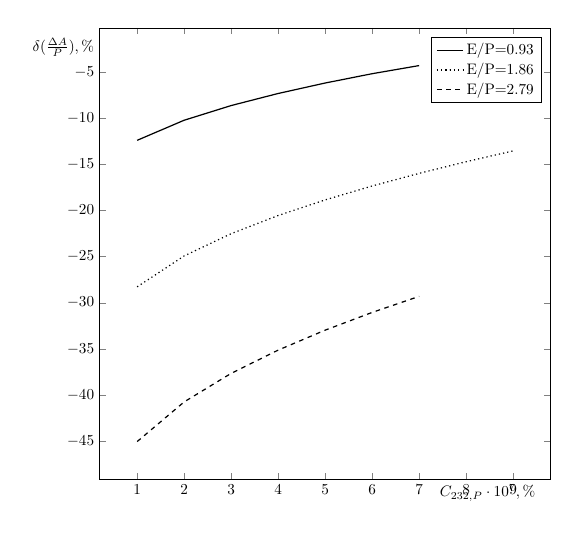
\begin{tikzpicture}[,
scale=0.55]
\begin{axis}[
  xlabel style = {{at={(axis description cs:.86,0)}}},
  ylabel = {$\delta(\frac{\Delta A}{P}), \%$},
  ylabel style = {{at={(axis description cs:-0.08,.925)},rotate=270,anchor=south}},
  xlabel = {$C_{232,P}\cdot10^{7}, \%$},
  width=12cm, height=12cm
]

\addplot+[mark=none,
  solid, black, thick
] coordinates {
  (1.0, -12.395218440946906)
  (2.0, -10.219020529323354)
  (3.0000000000000004, -8.626929870001328)
  (4.0, -7.3185844692402915)
  (5.0, -6.185264012646069)
  (6.0, -5.173768588868835)
  (7.000000000000001, -4.29293979177781)
};
\addlegendentry{{}{E/P=0.93}}

\addplot+[mark=none,
  dotted, black, thick
] coordinates {
  (1.0, -28.282242175940937)
  (2.0, -24.929077234925025)
  (3.0000000000000004, -22.516662376271356)
  (4.0, -20.550634890717415)
  (5.0, -18.85615249546271)
  (6.0, -17.34800036201673)
  (7.000000000000001, -15.978805541243855)
  (8.0, -14.71681616393461)
  (9.000000000000002, -13.541592549068923)
};
\addlegendentry{{}{E/P=1.86}}

\addplot+[mark=none,
  dashed, black, thick
] coordinates {
  (1.0, -45.057945429681226)
  (2.0, -40.758242565718376)
  (3.0000000000000004, -37.66157309459905)
  (4.0, -35.14302713983917)
  (5.0, -32.97793340752656)
  (6.0, -31.056144200883885)
  (7.000000000000001, -29.31422868906391)
};
\addlegendentry{{}{E/P=2.79}}

\end{axis}
\end{tikzpicture}


      \caption{{Зависимость экономии работы разделения от ПДК $^{232}$U в НОУ-продукте с обогащением на уровне 4,4\% для разных пропорций возврата урана.{\label{sw44}}}}
    \end{minipage}%
    \begin{minipage}{.5\textwidth}
      \centering
      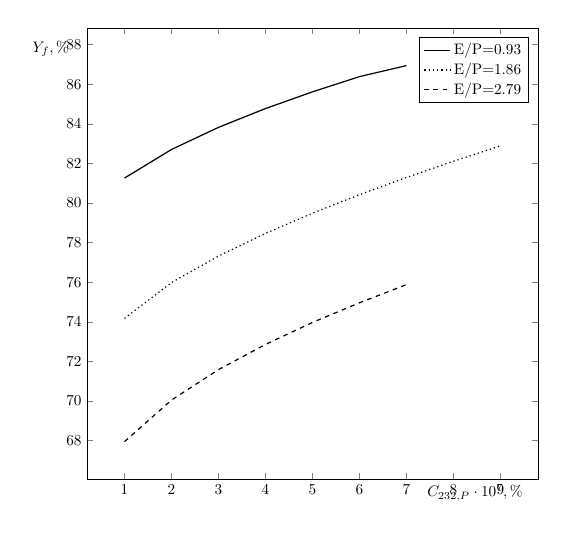
\begin{tikzpicture}[,
scale=0.55]
\begin{axis}[
  xlabel style = {{at={(axis description cs:.86,0)}}},
  ylabel = {$Y_{f}, \%$},
  ylabel style = {{at={(axis description cs:-0.08,.925)},rotate=270,anchor=south}},
  xlabel = {$C_{232,P}\cdot10^{7}, \%$},
  width=12cm, height=12cm
]

\addplot+[mark=none,
  solid, black, thick
] coordinates {
  (1.0, 81.2599146274243)
  (2.0, 82.70510635581616)
  (3.0000000000000004, 83.82183689954859)
  (4.0, 84.77127401369083)
  (5.0, 85.61487919146296)
  (6.0, 86.38356067088392)
  (7.000000000000001, 86.94074198596759)
};
\addlegendentry{{}{E/P=0.93}}

\addplot+[mark=none,
  dotted, black, thick
] coordinates {
  (1.0, 74.17655829999579)
  (2.0, 75.98498213201852)
  (3.0000000000000004, 77.32265969408223)
  (4.0, 78.46540402752339)
  (5.0, 79.48580928842689)
  (6.0, 80.42063662698051)
  (7.000000000000001, 81.29053109508794)
  (8.0, 82.1100269832236)
  (9.000000000000002, 82.88835691546974)
};
\addlegendentry{{}{E/P=1.86}}

\addplot+[mark=none,
  dashed, black, thick
] coordinates {
  (1.0, 67.95360281561639)
  (2.0, 70.05234164130057)
  (3.0000000000000004, 71.58870177419513)
  (4.0, 72.85958391192455)
  (5.0, 73.97031718490105)
  (6.0, 74.96387446964957)
  (7.000000000000001, 75.87957963032518)
};
\addlegendentry{{}{E/P=2.79}}

\end{axis}
\end{tikzpicture}


      \caption{{Зависимость степени извлечения $^{235}$U из регенерата от ПДК $^{232}$U в НОУ-продукте с обогащением на уровне 4,4\% для разных пропорций возврата урана.{\label{exR44}}}}
    \end{minipage}
\end{figure}


\begin{figure}
    \centering
    \begin{minipage}{.5\textwidth}
      \centering
      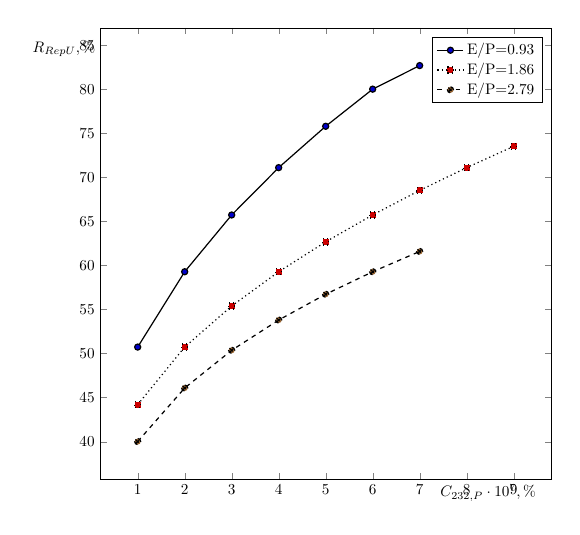
\begin{tikzpicture}[,
scale=0.55]
\begin{axis}[
  xlabel style = {{at={(axis description cs:.86,0)}}},
  ylabel = {$R_{RepU}, \%$},
  ylabel style = {{at={(axis description cs:-0.08,.925)},rotate=270,anchor=south}},
  xlabel = {$C_{232,P}\cdot10^{7}, \%$},
  width=12cm, height=12cm
]

\addplot+[
  solid, black, thick
] coordinates {
  (1.0, 50.745320366220234)
  (2.0, 59.30149726322195)
  (3.0000000000000004, 65.7519664106782)
  (4.0, 71.12954522207235)
  (5.0, 75.82763880377072)
  (6.0, 80.04430359281832)
  (7.000000000000001, 82.72459665893969)
};
\addlegendentry{{}{E/P=0.93}}

\addplot+[
  dotted, black, thick
] coordinates {
  (1.0, 44.20353110984807)
  (2.0, 50.745320366220234)
  (3.0000000000000004, 55.41327633341921)
  (4.0, 59.30149726322195)
  (5.0, 62.69903149138577)
  (6.0, 65.75196641067834)
  (7.000000000000001, 68.5430309981216)
  (8.0, 71.12954522207235)
  (9.000000000000002, 73.54852477832327)
};
\addlegendentry{{}{E/P=1.86}}

\addplot+[
  dashed, black, thick
] coordinates {
  (1.0, 40.009414250517715)
  (2.0, 46.09394772079198)
  (3.0000000000000004, 50.37816062607195)
  (4.0, 53.81590263606467)
  (5.0, 56.74369030977263)
  (6.0, 59.30149726322191)
  (7.000000000000001, 61.61037730716592)
};
\addlegendentry{{}{E/P=2.79}}

\end{axis}
\end{tikzpicture}


\caption{{Зависимость степени извлечения $^{235}$U из регенерата от ПДК $^{232}$U в НОУ-продукте с обогащением на уровне 4,4\% для разных пропорций возврата урана.{\label{exR44}}}}
    \end{minipage}%
    \begin{minipage}{.5\textwidth}
      \centering
      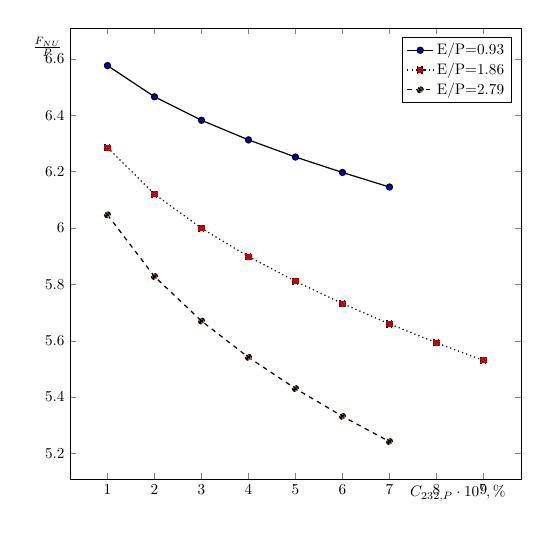
\begin{tikzpicture}[,
scale=0.55]
\begin{axis}[
  xlabel style = {{at={(axis description cs:.86,0)}}},
  ylabel = {$\frac{F_{NU}}{P}$},
  ylabel style = {{at={(axis description cs:-0.05,.925)},rotate=270,anchor=south}},
  xlabel = {$C_{232,P}\cdot10^{7}, \%$},
  width=12cm, height=12cm
]

\addplot+[
  solid, black, thick
] coordinates {
  (1.0, 6.575757299437289)
  (2.0, 6.465108289643847)
  (3.0000000000000004, 6.381756807732527)
  (4.0, 6.312192498795184)
  (5.0, 6.251327236245885)
  (6.0, 6.196612502667002)
  (7.000000000000001, 6.144912790012471)
};
\addlegendentry{{}{E/P=0.93}}

\addplot+[
  dotted, black, thick
] coordinates {
  (1.0, 6.28499725470176)
  (2.0, 6.119625794579712)
  (3.0000000000000004, 5.998819447555168)
  (4.0, 5.898327797408319)
  (5.0, 5.810535158754925)
  (6.0, 5.731623730169017)
  (7.000000000000001, 5.659437328483021)
  (8.0, 5.592496437975026)
  (9.000000000000002, 5.529842791100203)
};
\addlegendentry{{}{E/P=1.86}}

\addplot+[
  dashed, black, thick
] coordinates {
  (1.0, 6.046361666625544)
  (2.0, 5.827647612753036)
  (3.0000000000000004, 5.669693931908062)
  (4.0, 5.54091588676854)
  (5.0, 5.429941624846872)
  (6.0, 5.331547353770463)
  (7.000000000000001, 5.242056929548795)
};
\addlegendentry{{}{E/P=2.79}}

\end{axis}
\end{tikzpicture}


\caption{{Зависимость расхода природного урана от ПДК $^{232}$U в НОУ-продукте с обогащением на уровне 4,4\% для разных пропорций возврата урана.{\label{F0R44}}}}
    \end{minipage}
\end{figure}


\begin{figure}
    \centering
    \begin{minipage}{.5\textwidth}
      \centering
      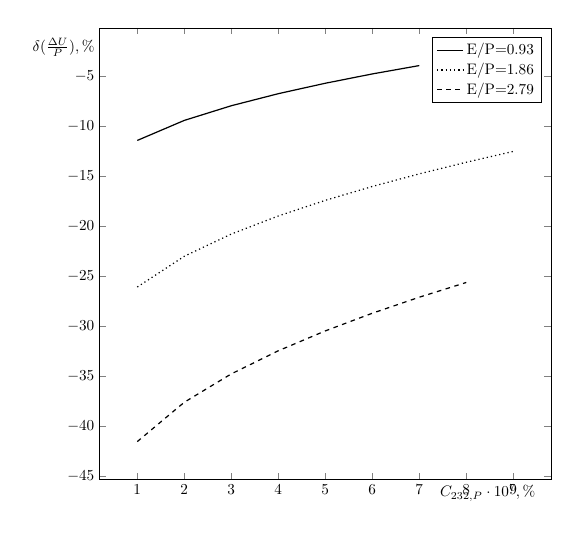
\begin{tikzpicture}[,
scale=0.55]
\begin{axis}[
  xlabel style = {{at={(axis description cs:.86,0)}}},
  ylabel = {$\delta(\frac{\Delta U}{P}), \%$},
  ylabel style = {{at={(axis description cs:-0.08,.925)},rotate=270,anchor=south}},
  xlabel = {$C_{232,P}\cdot10^{7}, \%$},
  width=12cm, height=12cm
]

\addplot+[mark=none,
  solid, black, thick
] coordinates {
  (1.0, -11.442050325962452)
  (2.0, -9.438723200431037)
  (3.0000000000000004, -7.9728246964313)
  (4.0, -6.768022196914314)
  (5.0, -5.7242794711367315)
  (6.0, -4.7922989130984135)
  (7.000000000000001, -3.956523255555432)
};
\addlegendentry{{}{E/P=0.93}}

\addplot+[mark=none,
  dotted, black, thick
] coordinates {
  (1.0, -26.09957395082424)
  (2.0, -23.022672963318332)
  (3.0000000000000004, -20.802863046158134)
  (4.0, -18.993519736891432)
  (5.0, -17.43387788617293)
  (6.0, -16.045572170953353)
  (7.000000000000001, -14.785062105867015)
  (8.0, -13.623128278493162)
  (9.000000000000002, -12.541001761914492)
};
\addlegendentry{{}{E/P=1.86}}

\addplot+[mark=none,
  dashed, black, thick
] coordinates {
  (1.0, -41.554133458995025)
  (2.0, -37.62214258113987)
  (3.0000000000000004, -34.78539667116384)
  (4.0, -32.475395453374304)
  (5.0, -30.487594682338603)
  (6.0, -28.721514147914533)
  (7.000000000000001, -27.11944341607787)
  (8.0, -25.644440494125277)
};
\addlegendentry{{}{E/P=2.79}}

\end{axis}
\end{tikzpicture}


\caption{{Зависимость экономии работы разделения от ПДК $^{232}$U в НОУ-продукте с обогащением на уровне 4,7\% для разных пропорций возврата урана.{\label{sw47}}}}
    \end{minipage}%
    \begin{minipage}{.5\textwidth}
      \centering
      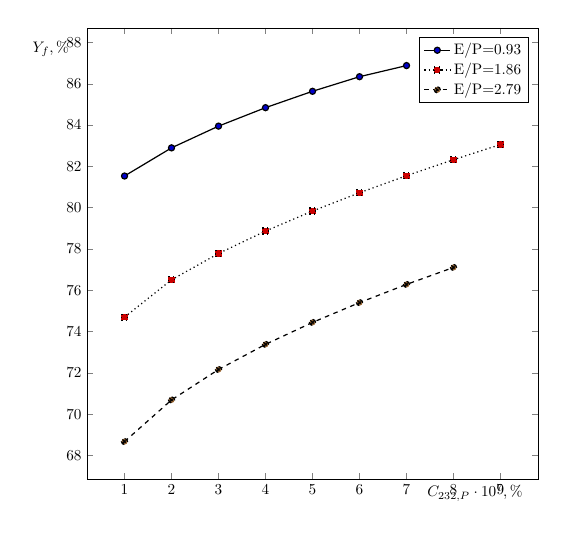
\begin{tikzpicture}[,
scale=0.55]
\begin{axis}[
  xlabel style = {{at={(axis description cs:.86,0)}}},
  ylabel = {$Y_{f}, \%$},
  ylabel style = {{at={(axis description cs:-0.08,.925)},rotate=270,anchor=south}},
  xlabel = {$C_{232,P}\cdot10^{7}, \%$},
  width=12cm, height=12cm
]

\addplot+[
  solid, black, thick
] coordinates {
  (1.0, 81.53156037359754)
  (2.0, 82.89545086273719)
  (3.0000000000000004, 83.9478345607235)
  (4.0, 84.84152401044177)
  (5.0, 85.63479347902604)
  (6.0, 86.3412156692256)
  (7.000000000000001, 86.88027992336104)
};
\addlegendentry{{}{E/P=0.93}}

\addplot+[
  dotted, black, thick
] coordinates {
  (1.0, 74.69415676339759)
  (2.0, 76.50476826786495)
  (3.0000000000000004, 77.77849512744808)
  (4.0, 78.86515635925242)
  (5.0, 79.83436020530084)
  (6.0, 80.72135365193532)
  (7.000000000000001, 81.54594313296484)
  (8.0, 82.32205886834831)
  (9.000000000000002, 83.05589060957709)
};
\addlegendentry{{}{E/P=1.86}}

\addplot+[
  dashed, black, thick
] coordinates {
  (1.0, 68.6697629941284)
  (2.0, 70.68575248489067)
  (3.0000000000000004, 72.15973261088106)
  (4.0, 73.37774759491083)
  (5.0, 74.44135268684659)
  (6.0, 75.39965734146578)
  (7.000000000000001, 76.28121651908731)
  (8.0, 77.10358771087932)
};
\addlegendentry{{}{E/P=2.79}}

\end{axis}
\end{tikzpicture}


\caption{{Зависимость степени извлечения $^{235}$U от ПДК $^{232}$U в НОУ-продукте с обогащением на уровне 4,7\% для разных пропорций возврата урана.{\label{ex47}}}}
\end{minipage}
\end{figure}

\begin{figure}
    \centering
    \begin{minipage}{.5\textwidth}
      \centering
      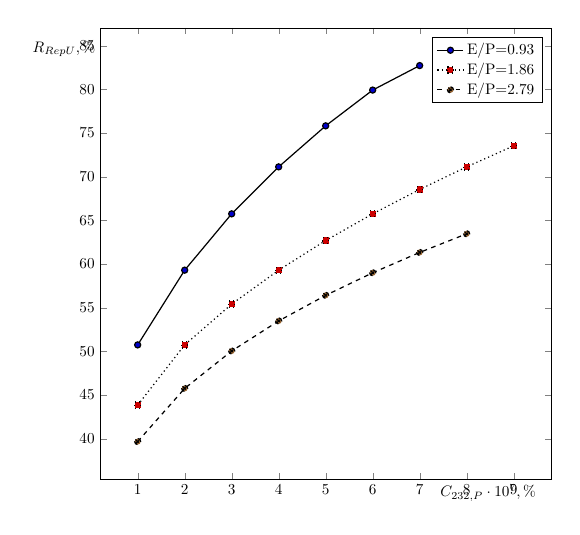
\begin{tikzpicture}[,
scale=0.55]
\begin{axis}[
  xlabel style = {{at={(axis description cs:.86,0)}}},
  ylabel = {$R_{RepU}, \%$},
  ylabel style = {{at={(axis description cs:-0.08,.925)},rotate=270,anchor=south}},
  xlabel = {$C_{232,P}\cdot10^{7}, \%$},
  width=12cm, height=12cm
]

\addplot+[
  solid, black, thick
] coordinates {
  (1.0, 50.74532036622023)
  (2.0, 59.30149726322195)
  (3.0000000000000004, 65.75196641067834)
  (4.0, 71.12954522207235)
  (5.0, 75.82763880377072)
  (6.0, 79.9222355420343)
  (7.000000000000001, 82.72736369212772)
};
\addlegendentry{{}{E/P=0.93}}

\addplot+[
  dotted, black, thick
] coordinates {
  (1.0, 43.8508093556669)
  (2.0, 50.745320366220234)
  (3.0000000000000004, 55.41327633341921)
  (4.0, 59.30149726322195)
  (5.0, 62.699031491385725)
  (6.0, 65.75196641067818)
  (7.000000000000001, 68.5430309981216)
  (8.0, 71.12954522207235)
  (9.000000000000002, 73.53797277442622)
};
\addlegendentry{{}{E/P=1.86}}

\addplot+[
  dashed, black, thick
] coordinates {
  (1.0, 39.675583995839325)
  (2.0, 45.761133085161255)
  (3.0000000000000004, 50.047914553011395)
  (4.0, 53.488618646439654)
  (5.0, 56.419645475250455)
  (6.0, 59.003049808125226)
  (7.000000000000001, 61.33254693680554)
  (8.0, 63.465686451699256)
};
\addlegendentry{{}{E/P=2.79}}

\end{axis}
\end{tikzpicture}


\caption{{Зависимость степени извлечения $^{235}$U из регенерата от ПДК $^{232}$U в НОУ-продукте с обогащением на уровне 4,7\% для разных пропорций возврата урана.{\label{exR47}}}}
    \end{minipage}%
    \begin{minipage}{.5\textwidth}
      \centering
      \begin{tikzpicture}[,
scale=0.55]
\begin{axis}[
  xlabel style = {{at={(axis description cs:.86,0)}}},
  ylabel = {$\frac{F_{NU}}{P}, \text{кг}$},
  ylabel style = {{at={(axis description cs:-0.12,.925)},rotate=270,anchor=south}},
  xlabel = {$C_{232,P}\cdot10^{7}, \%$},
  width=12cm, height=12cm
]

\addplot+[
  solid, black, thick
] coordinates {
  (1.0, 706.6354192785525)
  (2.0, 695.5705180447756)
  (3.0000000000000004, 687.235363636582)
  (4.0, 680.2789392306238)
  (5.0, 674.1924129651806)
  (6.0, 668.7266457264177)
  (7.000000000000001, 663.5511601107812)
};
\addlegendentry{{}{E/P=0.93}}

\addplot+[
  dotted, black, thick
] coordinates {
  (1.0, 677.959887355208)
  (2.0, 661.022268767328)
  (3.0000000000000004, 648.9416341028616)
  (4.0, 638.8924683215785)
  (5.0, 630.1132051976982)
  (6.0, 622.2220219123312)
  (7.000000000000001, 615.0034218929161)
  (8.0, 608.3093364348874)
  (9.000000000000002, 602.0503886358283)
};
\addlegendentry{{}{E/P=1.86}}

\addplot+[
  dashed, black, thick
] coordinates {
  (1.0, 654.2885822321769)
  (2.0, 632.4090216922981)
  (3.0000000000000004, 616.5981030031621)
  (4.0, 603.7017776368674)
  (5.0, 592.5838268649425)
  (6.0, 582.6875967531196)
  (7.000000000000001, 573.6906309431884)
  (8.0, 565.3894655334504)
};
\addlegendentry{{}{E/P=2.79}}

\end{axis}
\end{tikzpicture}


\caption{{Зависимость расхода природного урана от ПДК $^{232}$U в НОУ-продукте с обогащением на уровне 4,7\% для разных пропорций возврата урана.{\label{F0R47}}}}
\end{minipage}
\end{figure}


\begin{figure}
    \centering
    \begin{minipage}{.5\textwidth}
      \centering
      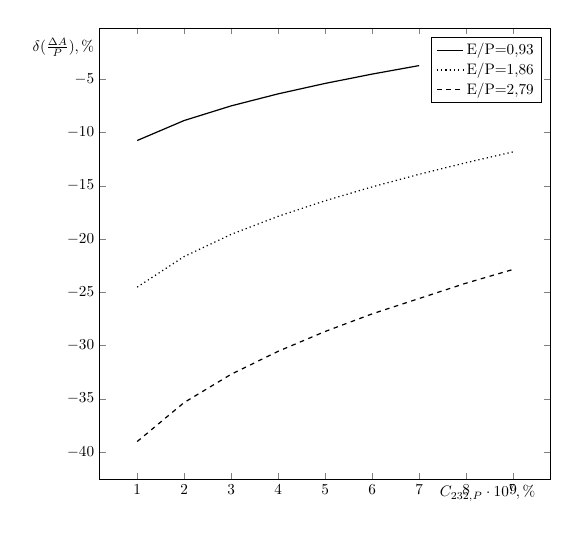
\begin{tikzpicture}[,
scale=0.55]
\begin{axis}[
  xlabel style = {{at={(axis description cs:.86,0)}}},
  ylabel = {$\delta(\frac{\Delta A}{P}), \%$},
  ylabel style = {{at={(axis description cs:-0.08,.925)},rotate=270,anchor=south}},
  xlabel = {$C_{232,P}\cdot10^{7}, \%$},
  width=12cm, height=12cm
]

\addplot+[mark=none,
  solid, black, thick
] coordinates {
  (1.0, -10.75592874548788)
  (2.0, -8.877549872366233)
  (3.0000000000000004, -7.50289958013979)
  (4.0, -6.3729908570898814)
  (5.0, -5.39405720345885)
  (6.0, -4.517136753769094)
  (7.000000000000001, -3.717964070419745)
};
\addlegendentry{{}{E/P=0,93}}

\addplot+[mark=none,
  dotted, black, thick
] coordinates {
  (1.0, -24.523693715258393)
  (2.0, -21.64946440952475)
  (3.0000000000000004, -19.56910789260241)
  (4.0, -17.87302824962024)
  (5.0, -16.41089275400384)
  (6.0, -15.109277255129713)
  (7.000000000000001, -13.927405951747463)
  (8.0, -12.837656298351746)
  (9.000000000000002, -11.820833744285492)
};
\addlegendentry{{}{E/P=1,86}}

\addplot+[mark=none,
  dashed, black, thick
] coordinates {
  (1.0, -39.02572435708815)
  (2.0, -35.35744140949972)
  (3.0000000000000004, -32.707361682832236)
  (4.0, -30.547279725027575)
  (5.0, -28.687040100935018)
  (6.0, -27.03315569727767)
  (8.0, -24.149000859531828)
  (9.000000000000002, -22.860928202940787)
};
\addlegendentry{{}{E/P=2,79}}

\end{axis}
\end{tikzpicture}


\caption{{Зависимость экономии работы разделения от ПДК $^{232}$U в НОУ-продукте с обогащением на уровне 4,95\% для разных пропорций возврата урана.{\label{sw495}}}}
    \end{minipage}%
    \begin{minipage}{.5\textwidth}
      \centering
      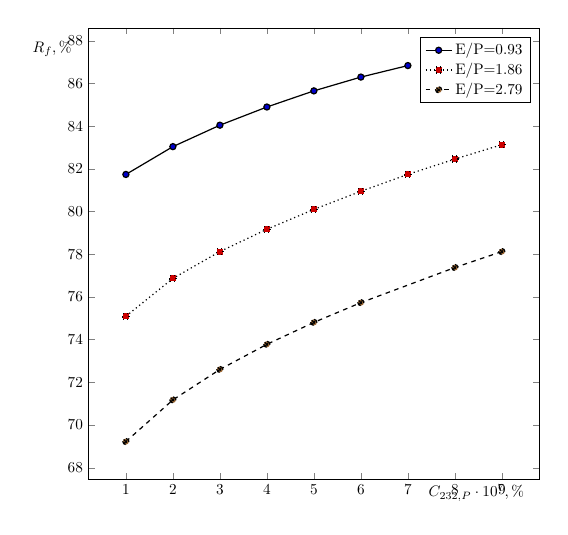
\begin{tikzpicture}[,
scale=0.55]
\begin{axis}[
  xlabel style = {{at={(axis description cs:.86,0)}}},
  ylabel = {$R_{f}, \%$},
  ylabel style = {{at={(axis description cs:-0.08,.925)},rotate=270,anchor=south}},
  xlabel = {$C_{232,P}\cdot10^{7}, \%$},
  width=12cm, height=12cm
]

\addplot+[
  solid, black, thick
] coordinates {
  (1.0, 81.73497884138504)
  (2.0, 83.03778477520555)
  (3.0000000000000004, 84.04194826713017)
  (4.0, 84.89394805905036)
  (5.0, 85.64964216184214)
  (6.0, 86.29627615264738)
  (7.000000000000001, 86.83475753524942)
};
\addlegendentry{{}{E/P=0.93}}

\addplot+[
  dotted, black, thick
] coordinates {
  (1.0, 75.09103641667504)
  (2.0, 76.86408581728926)
  (3.0000000000000004, 78.1230950450531)
  (4.0, 79.16703478387757)
  (5.0, 80.0973214088445)
  (6.0, 80.94802830843058)
  (7.000000000000001, 81.73831087619449)
  (8.0, 82.45610633767066)
  (9.000000000000002, 83.12799096181396)
};
\addlegendentry{{}{E/P=1.86}}

\addplot+[
  dashed, black, thick
] coordinates {
  (1.0, 69.22294832705394)
  (2.0, 71.17489372337026)
  (3.0000000000000004, 72.60072511995082)
  (4.0, 73.77803561909946)
  (5.0, 74.80542388393039)
  (6.0, 75.73053709257948)
  (8.0, 77.37433736075826)
  (9.000000000000002, 78.12192420776128)
};
\addlegendentry{{}{E/P=2.79}}

\end{axis}
\end{tikzpicture}


\caption{{Зависимость степени извлечения $^{235}$U от ПДК $^{232}$U в НОУ-продукте с обогащением на уровне 4,95\% для разных пропорций возврата урана.{\label{ex495}}}}
\end{minipage}
\end{figure}

\begin{figure}
    \centering
    \begin{minipage}{.5\textwidth}
      \centering
      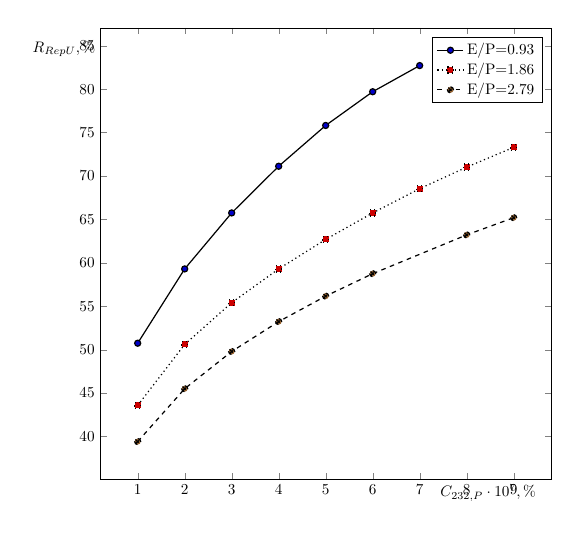
\begin{tikzpicture}[,
scale=0.55]
\begin{axis}[
  xlabel style = {{at={(axis description cs:.86,0)}}},
  ylabel = {$R_{RepU}, \%$},
  ylabel style = {{at={(axis description cs:-0.08,.925)},rotate=270,anchor=south}},
  xlabel = {$C_{232,P}\cdot10^{7}, \%$},
  width=12cm, height=12cm
]

\addplot+[
  solid, black, thick
] coordinates {
  (1.0, 50.745320366220234)
  (2.0, 59.30149726322195)
  (3.0000000000000004, 65.7519664106782)
  (4.0, 71.12954522207238)
  (5.0, 75.82763880377078)
  (6.0, 79.7135693705535)
  (7.000000000000001, 82.72543981227668)
};
\addlegendentry{{}{E/P=0.93}}

\addplot+[
  dotted, black, thick
] coordinates {
  (1.0, 43.577905794327634)
  (2.0, 50.60187689534774)
  (3.0000000000000004, 55.41327633341921)
  (4.0, 59.30149726322195)
  (5.0, 62.69903149138577)
  (6.0, 65.75196641067834)
  (7.000000000000001, 68.5430309981216)
  (8.0, 71.02486897820552)
  (9.000000000000002, 73.30720710112764)
};
\addlegendentry{{}{E/P=1.86}}

\addplot+[
  dashed, black, thick
] coordinates {
  (1.0, 39.414574744906304)
  (2.0, 45.501187547358626)
  (3.0000000000000004, 49.79017656124783)
  (4.0, 53.23340118139871)
  (5.0, 56.16715278135177)
  (6.0, 58.753339802423696)
  (8.0, 63.222220423599175)
  (9.000000000000002, 65.20220176963932)
};
\addlegendentry{{}{E/P=2.79}}

\end{axis}
\end{tikzpicture}


\caption{{Зависимость степени извлечения $^{235}$U из регенерата от ПДК $^{232}$U в НОУ-продукте с обогащением на уровне 4,95\% для разных пропорций возврата урана.{\label{exR495}}}}
    \end{minipage}%
    \begin{minipage}{.5\textwidth}
      \centering
      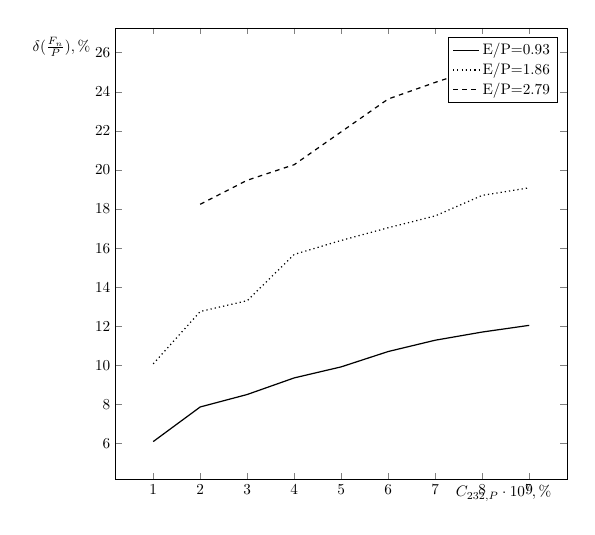
\begin{tikzpicture}[,
scale=0.55]
\begin{axis}[
  xlabel style = {{at={(axis description cs:.86,0)}}},
  ylabel = {$\delta(\frac{F_n}{P}), \%$},
  ylabel style = {{at={(axis description cs:-0.12,.925)},rotate=270,anchor=south}},
  xlabel = {$C_{232,P}\cdot10^{7}, \%$},
  width=12cm, height=12cm
]

\addplot+[mark=none,
  solid, black, thick
] coordinates {
  (1.0, 6.102609628967004)
  (2.0, 7.873257521230414)
  (3.0000000000000004, 8.510982187035465)
  (4.0, 9.359903696758797)
  (5.0, 9.924557345258734)
  (6.0, 10.709375471912841)
  (7.000000000000001, 11.287587970677283)
  (8.0, 11.705810902202751)
  (9.000000000000002, 12.048111265678951)
};
\addlegendentry{{}{E/P=0.93}}

\addplot+[mark=none,
  dotted, black, thick
] coordinates {
  (1.0, 10.07679447624098)
  (2.0, 12.756640615222503)
  (3.0000000000000004, 13.309773249935485)
  (4.0, 15.676539853992955)
  (5.0, 16.39235800951654)
  (6.0, 17.041722793102686)
  (7.000000000000001, 17.64593776461374)
  (8.0, 18.69753065296348)
  (9.000000000000002, 19.08456096001587)
};
\addlegendentry{{}{E/P=1.86}}

\addplot+[mark=none,
  dashed, black, thick
] coordinates {
  (2.0, 18.241079567317232)
  (3.0000000000000004, 19.47072745723193)
  (4.0, 20.268597025731783)
  (6.0, 23.628111214220738)
  (7.000000000000001, 24.476747414958155)
  (8.0, 25.273745846887998)
  (9.000000000000002, 25.337305198229632)
};
\addlegendentry{{}{E/P=2.79}}

\end{axis}
\end{tikzpicture}

\caption{{Зависимость расхода природного урана от ПДК $^{232}$U в НОУ-продукте с обогащением на уровне 4,95\% для разных пропорций возврата урана.{\label{F0R495}}}}
\end{minipage}
\end{figure}

    
На рисунках \ref{sw44}-\ref{F0R495} представлены кривые, отражающие зависимости от величины ограничения на концентрацию $^{232}$U в продукте следующих интегральных параметров каскадной схемы: $\delta(\frac{\Delta U}{P})$ -- экономия работы разделения по сравнению с ординарным каскадом, питаемым природным ураном, получающим продукт с эквивалентной эффективной концентрацией $^{235}$U (отрицательная величина означает перерасход работы разделения, а абсолютное значение, иными словами, соответствует потерям работы разделения, по сравнению с референтной схемы трехпоточного каскада для обогащения природного урана); степени извлечения $^{235}$U в схеме $R_f$ и из регенерата $R_{RepU}$, а также удельный расход природного урана $\frac{F_{NU}}{P}$ (на едицину продукта). На каждой из рисунков представлено по три кривые, каждая их которых отвечает одному из рассмотренных значений параметра ($E/P$).

Анализ графиков \ref{sw44}-\ref{F0R495} позволяет сделать заключение о применимости схемы двойного каскада с НОУ-разбавителем для задачи полного возврата массы регенерата в ядерный топливный цикл в условиях многократного рецикла как в условиях более жестких ограничений на содержание $^{232}U$, чем современные требования, так и при увеличении допустимого порога концентрации $^{232}U$ в НОУ-продукте. При этом снижение ограничений, которое может последовать за возможным изменением технологии процесса изготовления ТВЭЛов в будущем, позволяет улучшить интегральные параметры схемы. Аналогичный вывод о применимости схемы можно сделать и для случаев, предполагающих задействование двух и более единиц облученного топлива для производства одной единицы НОУ-продукта, так как производимый конечный продукт удовлетворяет заданным ограничениям на четные изотопы. Таким же образом схема показывает свою устойчивость для различных требуемых $^{235}$U эффективных значениях концентарции в продукте. Отметим, что решения задачи были найдены во всех случаях, кроме нескольких точках на кривой для случая ($E/P=0,93$), где не удалось найти решений при увеличении допустимой концентрации $^{232}U$ в товарном НОУ. Такой результат связан с тем, что в случае ($E/P=0,93$) входящая в каскадную схема масса $^{232}$U является наименьшей и даже, несмотря на относительную загрязнённость регенерата данным изотопом, его исходной массы недостаточно, чтобы получить концентрацию этого изотопа на уровне допустимого предела в товарном НОУ. Проще говоря, при $E/P=0,93$ невозможно найти решения, при которых концентрация $^{232}$U в товарном НОУ будет строго равна заданной предельной величине, а возможно только найти решения, для которых эта концентрация будет ниже. Естественно, получение концентрации $^{232}$U в продукте ниже допустимых пределов также можно рассматривать в качестве успешного решения поставленной задачи.  

В завершении еще раз подчеркнем, что исходя из анализа результатов, представленных на графиках \ref{sw44}-\ref{F0R495}, уменьшение допустимой концентрации $^{232}$U в продукте при фиксированном отношении исходного регенерата к товарному НОУ обусловливает ухудшение всех исследуемых ключевых показателей. Однако, из этих показателей, наиболее существенно падение степени извлечения $^{235}$U из регенерата при более строго ограничении на $^{232}$U, тогда как значительного увеличения расхода природного урана, увеличения числа центрифуг в каскадной схем (работы разделения), или значимого ухудшения извлечения $^{235}$U в схеме не наблюдается. И, самое главное, каскадная схема позволяет решить поставленную задачу для всех случаев.


\section{Общие выводы по результатам анализа схемы двойного каскада с НОУ-разбавителем}

В качестве обобщающих выводов по результатам анализа предложенной схемы двойного каскада с НОУ-разбавителем (рис. \ref{p2left}), обозначим следующее:
\begin{enumerate}
    \item схема применима для обогащения регенерированного урана в условиях многократного рецикла урана в топливе легководных реакторов, поскольку позволяет получать продукт, отвечающий всем требованиям на концентрации четных изотопов для регенерата различного исходного состава, включая рециклы, к которым накопилось повышенное содержание четных изотопов (на примере пятого рецикла);
    \item схема показывает свою устойчивость в условиях изменения внешних ограничений и требований к получаемому продукту;
    \item схема позволяет отделить участки обогащения регенерированного урана (где разделительное оборудование будет подвержено загрязнению минорными изотопами) от каскадов, обогащающих не содержащий $^{232,236}$U природный уран или ОГФУ. При этом доля разделительных мощностей, отводимых под работу с регенерированным ураном при наработке НОУ для загрузки реактора составляет не более 10\%;
     \item в схеме происходит накопление побочно производимого материала -- высокоактивного отхода (отбор второго каскада), в котором к тому же происходит потеря делящегося $^{235}$U. Стратегии дальнейшего обращения с данным отходом требуют отдельного анализа, который будет проведен далее в Главе 4.
    \item работа схемы связана с потерями работы разделения при двух этапах производственного процесса:
    \begin{enumerate}
        \item обеднение отбора первого каскада $P_1$ во втором каскаде;
        \item смешивание потоков $W_2$ с НОУ-разбавителем $P_0$, в которых различается содержание изотопа $^{235}$U;
    \end{enumerate}
\end{enumerate}






\section{Рассмотрение различных возможностей утилизации легкой фракции второго каскада в схеме}

\subsection{Анализ возможности утилизации легкой фракции путем ее перемешивания с регенератом, поступающим на обогащение}

\subsubsection{Описание схемы двойного каскада с НОУ-разбавителем с возвратом потока $P_2$ в цикл}

В качестве модификации каскадной схемы, представленной на рис. \ref{P2utilizationRing} предложен способ, позволяющий вернуть поток $P_2$ в топливный цикл для производства НОУ-продукта (рис. \ref{p2left}) \cite{nevinicaToplivnyyCiklLegkovodnogo2019, nevinicaSposobIzotopnogoVosstanovleniya2019}. Принцип ее работы состоит в следующем.

\begin{figure}[ht]
    \centerfloat{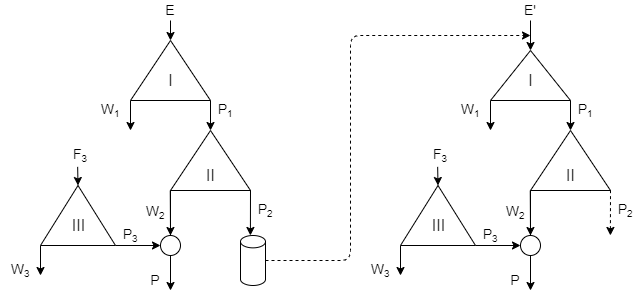
\includegraphics[scale=0.6]{cascades/P2utilizationRing}}
    \caption{Схема передачи загрязненной изотопом $^{232}$U фракции гексафторида урана в двойном каскаде от первой партии дообогащенного регенерированного урана к последующей. Обозначения: $E$ -- поток регенерированного урана; $P_1$ -- поток отбора первого каскада, выступающий питанием второго каскада; $P_2$ -- поток отбора второго каскада; $W_1$ -- поток отвала первого каскада; $W_2$ -- поток тяжелой фракции (условный «отвал») второго каскада; $P_0$ -- поток НОУ-разбавителя; $P$ -- финальный продукт (товарный низкообогащенный уран (НОУ), который подается на питание последующего двойного каскада, перемешиваясь с регенератом очередного рецикла}\label{P2utilizationRing}
\end{figure}

Учитывая, что каскадная схема двойного каскада с НОУ-разбавителем (рис. \ref{p2left}) предназначена для обогащения регенерата с высоким накопившимся в ходе серии пройденных рециклов содержанием изотопа $^{232}$U, можно использовать такую каскадную схему для вовлечения ранее полученного в потоке отбора второго каскада фракции $P_2$ загрязненной изотопом $^{232}$U. Выведенный ранее из системы гексафторида урана может быть перемешан с регенератом, полученным из следующей партии отработавшего топлива, то есть с составом более загрязненным изотопами $^{232,233,234,236}$U, чем исходно использовавшийся состав, побочным продуктом которого оказался этот $P_2$. Полученная таким образом в результате смешения $P_2$ предыдущего рецикла и регенерата очередного рецикла смесь будет отправлена на последующее обогащение (рис. \ref{P2utilizationRing}).

При использовании подобной схемы удастся полностью замкнуть топливный цикл по урану, а единственным отходом производства останется ОГФУ, образующийся в отвале первого каскада, который можно считать штатным отходом обогатительного производства с отработанными технологиями хранения и переработки. При этом после завершения производственного цикла останется невостребованным только та масса обогащенного по изотопу $^{232}$U гексафторида урана (загрязненной фракции легкого конца второго каскада (рис. \ref{P2utilizationRing})), которая будет образована после обогащения последней партии регенерата. Таким образом, предложенный подход к дообогащению регенерата урана позволяет организовать полный возврат массы регенерированного урана в топливный цикл в течение всего жизненного цикла задействованного урана.

При схожем наборе достоинств и недостатков схемы двойного каскада с НОУ-разбавителем с возвратом потока $P_2$ в цикл (рис. \ref{P2utilizationRing}), достоинством схемы с возвратом $P_2$ является более глубокая выработка потенциала делящегося $^{235}$U, накапливаемого совместно с изотопами $^{232,233,234}$U в загрязненной фракции второго каскада. Это позволяет добиваться меньших потерь $^{235}$U на всем жизненном цикле используемого урана.



Как видно из данных табл. \ref{vest2019_2} предложенная схема рециклирования действительно позволяет полностью израсходовать и исходный регенерированный уран и образующийся в результате использования двойного каскада высокообогащенный отход.

Итак, опираясь на результаты расчетов, можно сделать общие выводы касаемо двойного каскада с НОУ-разбавителем с возвратом потока $P_2$ в цикл:

\begin{enumerate}
    \item схема принципиально применима для обогащения регенерированного урана в условиях многократного рецикла урана в топливе легководных реакторов, поскольку позволяет получать продукт, отвечающий всем требованиям по концентрациям четных изотопов для регенерата различного исходного состава;
    \item достоинством схемы является полное отсутствие потерь $^{235}$U (не считая потока отвала первого каскада) в процессе рециклирования, а также полное отсутствие нештатного отхода вплоть до последней перегрузки последнего рецикла; Однако, ввиду искусственного повышения содержания четных изотопов $^{232,234}$U в получаемом продукте с каждой последующей перегрузкой возрастает масса отхода  $P_2$ и, соответственно, масса концентрирующегося в нем изотопа $^{235}$U, что уменьшает эффект от возврата изотопа $^{235}$U в цикл из-за его потерь вследствие увеличения потока загрязненной фракции, которое происходит вследствие роста концентраций четных изотопов в исходной смеси.
    \item возврат фракции отхода (потока $P_2$) в схему является причиной монотонного роста концентраций четных изотопов, что приводит к необходимости увеличения уровня обогащения получаемого НОУ и, тем самым, к росту затрат работы разделения, а также повышению концентрации изотопа $^{235}$U в НОУ-разбавителе ввиду необходимости компенсации влияния $^{236}$U;
    \item в схеме присутствуют потери работы разделения из-за необходимости обеднять отбор второго ординарного каскада $P_2$ в последующей составной каскадной схеме;
\end{enumerate}


В качестве общего вывода по результатам анализа схемы двойного каскада с НОУ-разбавителем с возвратом $P_2$ в топливный цикл (рис. \ref{p2left}) представим следующее:
\begin{enumerate}
    \item схема применима для обогащения регенерированного урана в условиях многократного рецикла урана в топливе легководных реакторов, поскольку позволяет получать продукт, отвечающий всем требованиям на концентрации четных изотопов на основе состава регенерата с повышенным исходным содержанием изотопов $^{232,234}$U, который не позволяет решить проблему с помощью ординарного каскада;
    \item схема позволяет использовать поток «легкой» фракции второго каскада ($P_2$), поскольку указанный поток возвращается в топливный цикл, что снимает проблемы его долговременного хранения и связанные с ним затраты;
    \item схема c возвратом $P_2$ как и предшествующая схема без возврата $P_2$, подходит для решения задачи обогащения урана при одновременном выполнении всех сопутствующих условий, в том числе, при обогащении регенерированного урана, прошедшего несколько последовательных рециклов;
    \item схема c возвратом $P_2$ как и предшествующая схема двойного каскада с НОУ-разбавителем, позволяет задействовать для воспроизводства ядерного топлива накопленный в значительных количествах обедненный уран. Производимый ею отвал регенерированного урана ($W_1$) имеет содержание четных изотопов на уровне ниже допустимых ограничений. Это позволяет говорить о том, что такие отвалы могут безопасно длительно хранится в виде гексафторида урана или быть переработанными на установке дефторирования;
    \item в схеме на трех стадиях процесса обогащения происходят потери работы разделения:
    \begin{enumerate}
        \item обеднение отбора первого каскада $P_1$ во втором каскаде;
        \item смешивание потоков $W_2$ с НОУ-разбавителем $P_0$, в которых различается содержание изотопа $^{235}$U;
        \item смешивания потоков $P_2$ и $E$ на входе в каскады, принимающие регенерат последующих рециклов (начиная с третьего).
    \end{enumerate}
    \item в схеме, как и в предшествующей немодифицированной схеме двойного каскада с НОУ-разбавителем, физически разделены участки каскада с разделительным оборудованием, пропускающие через себя регенерированный урана (первые два каскады, принимающие на вход поток $E$ на рисунке \ref{P2utilizationRing}) и участок обогащения сырья для наработки НОУ-разбавителя -- природного или обедненного урана -- материалов, которые не загрязнены четными изотопами $^{232,236}$U. В дальнейшем это позволит задействовать оборудование каскада, использовавшегося для наработки разбавителя, в операциях обогащения природного урана или другого сырьевого материала, не загрязненного четными изотопами, а значит в менее жестконормированных условиях эксплуатации;
    \item практическая реализация представляется нецелесообразной, поскольку данная схема не дает ощутимых преимуществ с точки зрения интегральной экономии $^{235}$U в топливном цикле по отношению к схеме двойного каскада с НОУ-разбавителем (рис. \ref{p2left}), причем реализации схемы с возвратом $P_2$ возможна только в условиях непрерывной работы реактора и постоянного поступления новых партий регенерата на дообогащение.
\end{enumerate}



Заметим, что процесс возврата данного материала в воспроизводство низкообогащенного урана может быть начат также и после дообогащения регенерата уже для одной ТВС и даже для ее части (непрерывный возврат). В этом случае также удастся полностью замкнуть топливный цикл по урану, а единственным отходом производства станет обедненный гексафторид, образующийся в отвале первого каскада, который можно считать штатным отходом обогатительного производства, для которого на сегодняшний день отработаны технологии хранения и переработки.

При этом после вывода завода из эксплуатации (или остановки на планово-предупредительный ремонт) останется невостребованным только та масса обогащенного по изотопу $^{232}$U гексафторида урана, которая будет образована после обогащения последней партии регенерата на этом заводе. Таким образом, рассматриваемый подход к дообогащению регенерата урана позволяет организовать полный возврат регенерированного урана в топливный цикл в течение практически всего жизненного цикла топлива легководных реакторов, работающих в замкнутом топливном цикле.

Несмотря на очевидные достоинства рассматриваемого способа, возникает вопрос о его эффективности с точки зрения интегральных характеристик разделительного каскада, важных для экономики топливного цикла в целом. Речь идет об экономии природного урана в цикле и затратах работы разделения на единицу массы готового НОУ.
В связи с этим целью настоящей работы явилась оценка интегральных показателей для рассматриваемой схемы в условиях ее использования для обогащения регенерированного урана и наработки НОУ для обеспечения поставок для формирования топлива нескольких последовательных загрузок реактора.

Исходный регенерат второго рецикла использован для производства тепловыделяющих сборок (ТВС) c обогащением: 4,95\%. Из указанного состава изготавливают сначала топливо для первой перегрузки. Далее, загрязненную фракцию от обогащения регенерата для первой перегрузки перемешивают с регенератом исходного состава для второго рецикла и направляют на последующее обогащение для получения топлива следующей перегрузки. Всего рассмотрено 7 перегрузок. При расчете состава низкообогащенного урана после каскада при получении топлива для каждой из перегрузок решается оптимизационную задачу (метод прямого поиска) для шести выбранных критериев эффективности при шаге по концентрации в потоке отбора первого каскада и потоках отбора и отвала второго каскада равном 1\%. Для сопоставления отбирали только те варианты, для которых выполнены описанные выше условия для концентраций четных изотопов. Диапазоны варьирования концентраций в выходящих потоках каскадной схемы были следующими. Концентрацию $^{235}$U в первом каскаде варьировали в диапазоне 7-17\%, в отвале второго каскада 6-16\%, в отборе второго каскада 10-20\%.

Ввиду сложности многокритериального анализа для каждой из перегрузок был рассмотрен случай с параллельными «ветками», на каждой из которых проводили последовательный расчет изотопных составов и параметров разделительного каскада для семи перегрузок, при условии оптимизации на каждом из шагов по одному и тому же критерию эффективности. В качестве критериев эффективности выступали величины: (1) минимум расхода природного урана на единицу продукта, (2) минимум затрат работы разделения на единицу продукта, (3) минимум концентрации изотопа $^{232}$U (в диапазоне 2-$5\cdot10^{-7}$\%), (4) минимум концентрации изотопа $^{236}$U, (5) минимум массы отхода двойного каскада, (6) максимум степени извлечения $^{235}$U из поступающего в обогащение регенерата. Под степенью извлечения $^{235}$U из исходного регенерированного урана понимали отношение массы $^{235}$U в отвале второго каскада к массе $^{235}$U в исходной смеси регенерата, поступившего для обогащения.

Далее представлены результаты проведенных вычислительных экспериментов и проведен их анализ. 
На рисунке \ref{3} представлено изменение удельного расхода природного урана при получении товарного НОУ при шести различных критериях эффективности, по которым осуществляли оптимизацию для каждой перегрузки. Как следует из анализа зависимостей, показанных на указанном рисунке при оптимизации по четырем, а именно: минимуму удельного расхода природного урана, минимуму удельных затрат работы разделения, минимуму массы отхода двойного каскада, максимуму степени извлечения $^{235}$U из поступающего в обогащение регенерата, зависимости практически совпадают. Это можно объяснить тем, что данные критерии близки по своей сути. Например, максимум степени извлечения $^{235}$U из поступающего в обогащение регенерата должен приводить к необходимости использования минимальной массы $^{235}$U из природного сырья, что и выражается в уменьшении расхода природного сырья. В целом все кривые представляют собой уменьшающиеся функции, что логично, учитывая, что с каждой перегрузкой масса исходного регенерата возрастает одновременно с повышением концентрации $^{235}$U в нем. Однако при использовании в качестве критериев эффективности минимумов концентраций $^{232}$U и $^{236}$U в товарном НОУ соответствующие кривые заметно отличаются от четырех упомянутых выше случаев. Как можно видеть из рисунка \ref{3} (кривые 4 и 5) для этих случаев характерен заметно больший расход природного урана. Данный факт можно объяснить тем, что при оптимизации по минимуму концентраций четных изотопов в товарном НОУ происходит «вытеснение» четных изотопов, а вместе с ними и значительной массы $^{235}$U в отбор второго каскада. В результате заметно падает степень извлечения $^{235}$U из исходного регенерата (рисунок \ref{4}) и масса отхода, что отчетливо заметно по зависимостям на рисунке \ref{5}, в соответствии с которыми масса отхода для этих критериев на последних перегрузках превышает массу исходного регенерата и составляет величину более 30\% от массы исходного регенерата. В то время как для других критериев эта величина даже на 7-й перегрузке не превышает 10\%. Общей закономерностью для всех случаев является снижение расхода природного сырья с каждой перегрузкой (рисунок \ref{6}).


\begin{figure}[ht]
    \begin{minipage}{.5\textwidth}
      \centering
      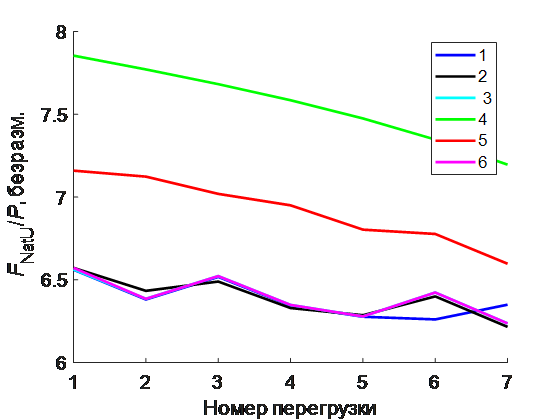
\includegraphics[width=.8\linewidth]{images/net/3}  
      \caption{Изменение величины удельного расхода природного урана в двойном каскаде с замыканием в зависимости от номера перегрузки для обогащения 4,95\% для различных критериев эффективности.}
      \label{3}
    \end{minipage}
    \begin{minipage}{.5\textwidth}
      \centering
      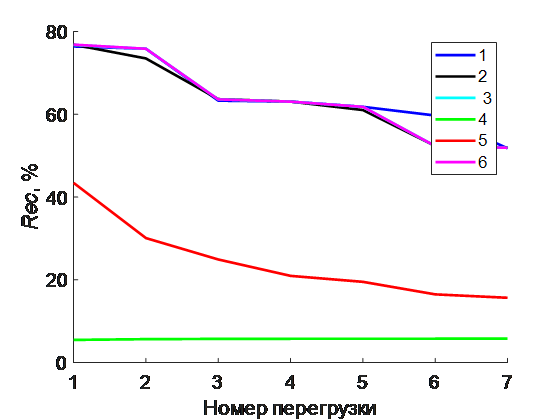
\includegraphics[width=.8\linewidth]{images/net/4}  
      \caption{Степень извлечения $^{235}$U из исходного регенерата в зависимости от номера перегрузки для обогащения 4,95\% для различных критериев эффективности.}
      \label{4}
    \end{minipage}
    \begin{minipage}{.5\textwidth}
      \centering
      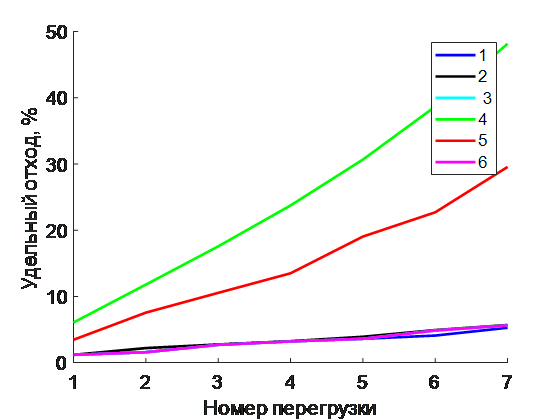
\includegraphics[width=.8\linewidth]{images/net/5}  
      \caption{Величину удельного отхода (на единицу исходного регенерата) в зависимости от номера перегрузки для обогащения 4,95\% для различных критериев эффективности.}
      \label{5}
    \end{minipage}
    \begin{minipage}{.5\textwidth}
      \centering
      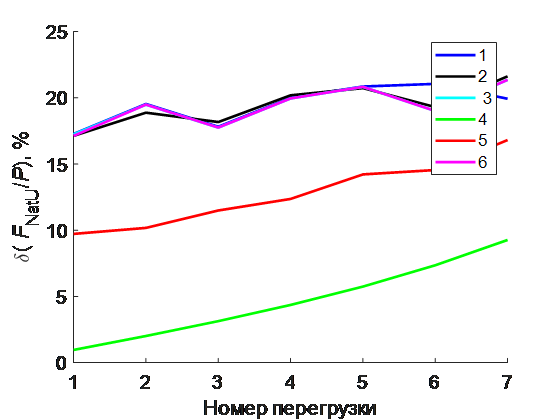
\includegraphics[width=.8\linewidth]{images/net/6}  
      \caption{Относительное изменение величины удельного расхода природного урана в двойном каскаде с замыканием в зависимости от номера перегрузки для обогащения 4,95\% для различных критериев эффективности.}
      \label{6}
    \end{minipage}
\end{figure}


Обозначения для рис. \ref{3}–\ref{6} приняты следующие. Кривая 1: оптимумы по расходу природного урана, кривая 2: оптимумы по затратам работы разделения, кривая 3: оптимумы по массе высокообогащенной фракции, кривая 4: минимум концентрации $^{232}$U, кривая 5: минимум концентрации $^{236}$U, кривая 6: максимум степени извлечения минимум $^{235}$U из регенерата урана.

В результате описанных выше процессов увеличивается и достигает значений, близких к 2, величина отношения (исходный регенерат)/продукт (риc. \ref{7}). Анализ зависимостей концентраций $^{235}$U и четных изотопов в регенерате, поступающем на обогащение после смешивания с высокообогащенной фракцией показывает, что все они повышается с каждой перегрузкой (рисунки \ref{8}–\ref{11}). Однако при использовании в качестве критериев эффективности минимумов концентраций  $^{232}$U и  $^{236}$U в товарном НОУ концентрации всех указанных выше изотопов в исходном регенерате возрастают заметно интенсивнее. Важно при этом отметить, что на последних перегрузках концентрация $^{235}$U в исходном регенерате превышает величину, требуемую для финального продукта (рисунок \ref{11}). Это означает, что схема начинает обеднять смесь и «чистить» ее от четных, а не обогащать. Особенно сильно это проявляется при минимизации концентраций четных изотопов в продукте, поскольку в этих случаях концентрация $^{235}$U в исходном регенерате могут приближаться к 5\% (рисунок \ref{10}). Подобные результаты говорят, в первую очередь, о нецелесообразности использования схемы в таком варианте для последовательного обогащения регенерата нескольких перегрузок с использованием в качестве критериев эффективности на каждом шаге требования минимальности концентраций $^{232}$U и  $^{236}$U в товарном НОУ. Однако требуют дополнительных исследований возможности дальнейшей модификации предложенной схемы, в том числе, для более эффективного использования исходного регенерата с повышенным содержанием $^{235}$U. Одним из таких вариантов может стать расширение диапазона увеличения концентрации  $^{235}$U в схеме, например, до 90\%. Другие варианты могут быть основаны на введении дополнительных потоков для разбавления четных изотопов и снижения концентрации  $^{235}$U до нужных значений.

\begin{figure}[ht]
    \centerfloat{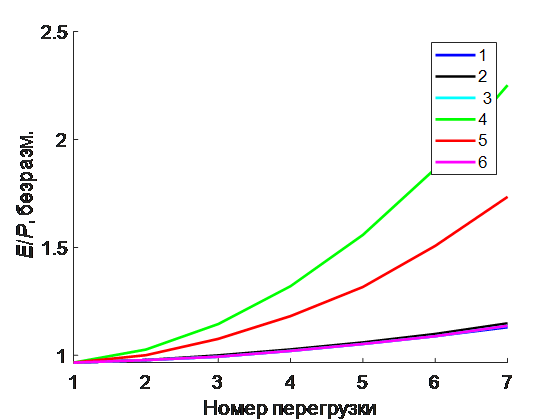
\includegraphics[scale=0.7]{images/net/7}}
    \caption{Зависимость отношения потоков исходного регенерата и финального продукта (товарного НОУ) от номера перегрузки для обогащения 4,95\% для различных критериев эффективности.}\label{7}
\end{figure}

\begin{figure}[ht]
    \begin{minipage}{.5\textwidth}
      \centering
      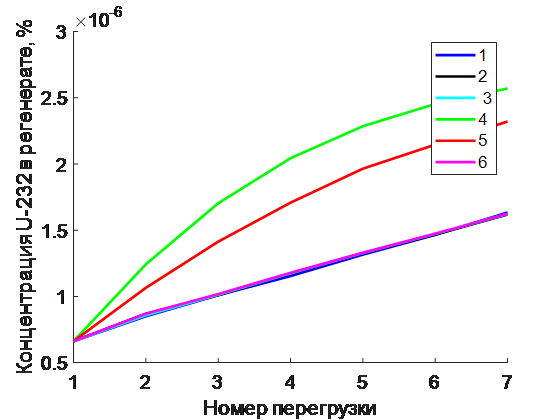
\includegraphics[width=.8\linewidth]{images/net/8}  
      \caption{Зависимость концентрации $^{232}$U в исходном регенерате от номера перегрузки для обогащения 4,95\% для различных критериев эффективности.}
      \label{8}
    \end{minipage}
    \begin{minipage}{.5\textwidth}
      \centering
      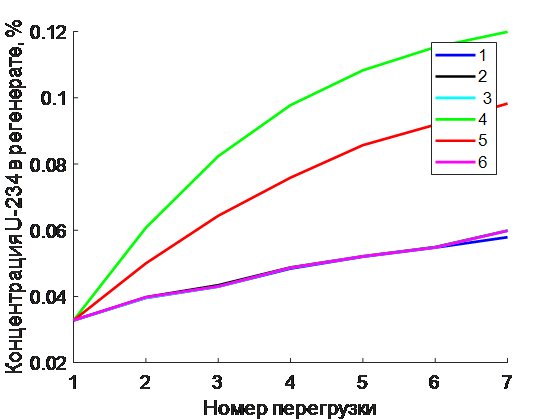
\includegraphics[width=.8\linewidth]{images/net/9}  
      \caption{Зависимость концентрации $^{234}$U в исходном регенерате от номера перегрузки для обогащения 4,95\% для различных критериев эффективности.}
      \label{9}
    \end{minipage}
    \begin{minipage}{.5\textwidth}
      \centering
      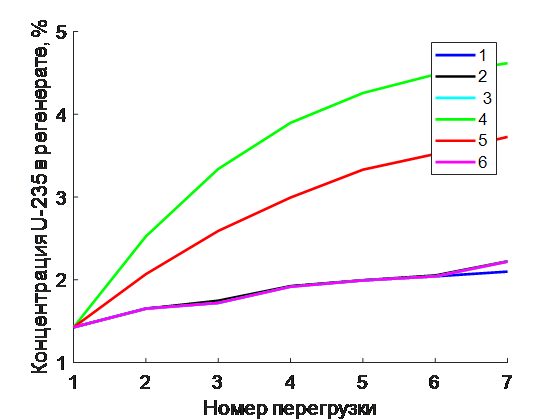
\includegraphics[width=.8\linewidth]{images/net/10}  
      \caption{Зависимость концентрации $^{235}$U в исходном регенерате от номера перегрузки для обогащения 4,95\% для различных критериев эффективности.}
      \label{10}
    \end{minipage}
    \begin{minipage}{.5\textwidth}
        \centering
        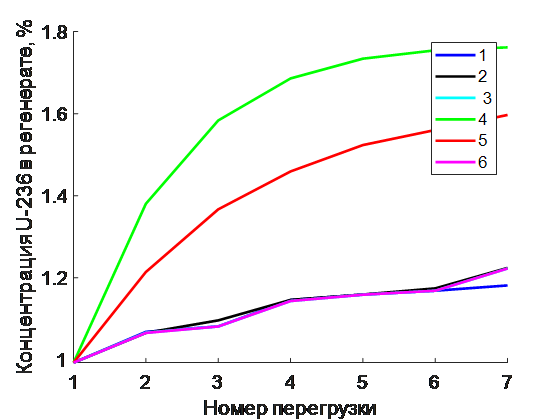
\includegraphics[width=.8\linewidth]{images/net/11}  
        \caption{Зависимость концентрации $^{236}$U в исходном регенерате от номера перегрузки для обогащения 4,95\% для различных критериев эффективности.}
        \label{11}
      \end{minipage}
\end{figure}

Обозначения для рис. \ref{7}–\ref{11} приняты следующие. Кривая 1: оптимумы по расходу природного урана, кривая 2: оптимумы по затратам работы разделения, кривая 3: оптимумы по массе высокообогащенной фракции, кривая 4: минимум концентрации $^{232}$U, кривая 5: минимум концентрации $^{236}$U, кривая 6: максимум степени извлечения минимум $^{235}$U из регенерата урана), E – поток питающего каскадную схему регенерата, P -- товарный НОУ.


Анализ изменения величины затрат работы разделения в зависимости от номера перегрузки и выбранного критерия эффективности показывает следующее. Для всех критериев, кроме случаев минимизации концентрации $^{232}$U или $^{236}$U затраты работы разделения сохраняются на определенном уровне, незначительно отличающемся от случая обогащения природного урана до соответствующей концентрации (рисунок \ref{12}). С увеличением номера перегрузки происходит незначительное снижение потерь работы разделения для этих случаев: с $\approx$5\% до $\approx$10\% (рисунок \ref{13}). При этом в случае минимизации концентраций изотопов $^{232}$U или $^{236}$U затраты работы разделения значительно выше и  могут на десятки процентов превосходить аналогичные затраты для случая обогащения природного урана для получения эквивалентного количества требуемого НОУ.

\begin{figure}[ht]
    \begin{minipage}{.5\textwidth}
      \centering
      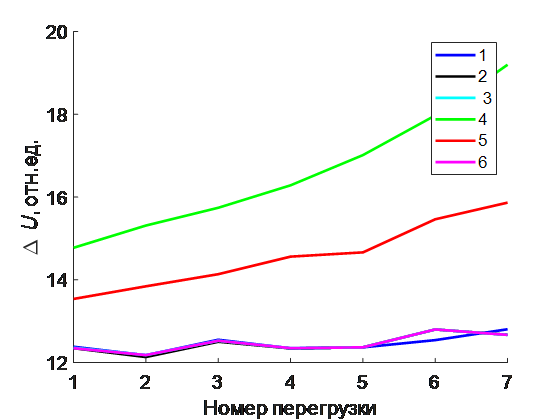
\includegraphics[width=.8\linewidth]{images/net/12}  
      \caption{Изменение величины удельных затрат работы разделения в двойном каскаде с замыканием в зависимости от номера перегрузки для обогащения 4,95\% для различных критериев эффективности.}
      \label{12}
    \end{minipage}
    \begin{minipage}{.5\textwidth}
      \centering
      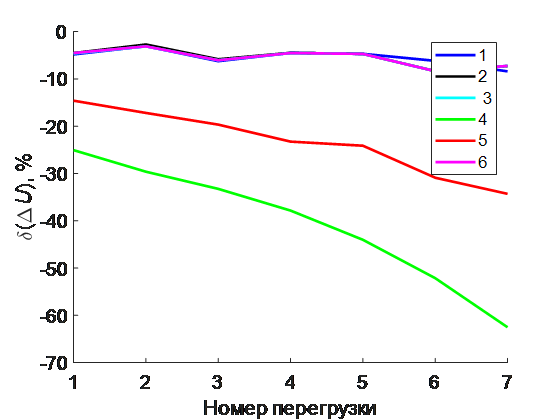
\includegraphics[width=.8\linewidth]{images/net/13}  
      \caption{Относительное изменение величины удельных затрат работы разделения в двойном каскаде с замыканием в зависимости от номера перегрузки для обогащения 4,95\% для различных критериев эффективности.}
      \label{13}
    \end{minipage}
\end{figure}

Обозначения для рис. \ref{12}–\ref{13} приняты следующие. Кривая 1: оптимумы по расходу природного урана, кривая 2: оптимумы по затратам работы разделения, кривая 3: оптимумы по массе высокообогащенной фракции, кривая 4: минимум концентрации $^{232}$U, кривая 5: минимум концентрации $^{236}$U, кривая 6: максимум степени извлечения минимум $^{235}$U из регенерата урана.

Рассматриваемая каскадная схема может работать в широком диапазоне изменения концентраций компонентов, в первую очередь, четных изотопов и $^{235}$U в исходном регенерате. Данный факт открывает возможности для применения схемы в условиях топливных циклов с увеличенной длительностью топливного цикла, а также в условиях многократного рецикла урана.

В зависимости от выбранного критерия эффективности для оптимизации схемы при расчете изотопного состава НОУ для каждой новой перегрузки, возможно обеспечить широкую вариативность параметров рассматриваемой каскадной схемы. При этом в случае выбора в качестве критериев эффективности величин удельного расхода природного урана, удельных затрат работы разделения, массы получаемого отхода или величины степени извлечения $^{235}$U из исходного регенерата оптимальные параметры схемы меняются незначительно. В то время, как при использовании в качестве критериев эффективности условий минимума концентраций $^{232}$U и $^{236}$U в товарном НОУ ключевые характеристики каскадов значительно отличаются от других критериев.

С ростом номера перегрузки происходит последовательно уменьшение расхода природного урана и затрат работы разделения. При этом на последних перегрузках экономия природного урана достигает величины 20\% и более. Это означает, что экономия природного урана в цикле в среднем будет примерно на треть выше типичного значения в 15\%. Причиной этому более эффективное использование $^{235}$U из регенерата.




\subsection{Анализ возможности утилизации легкой фракции путем ее перемешивания с обедненным ураном и последующим обогащением}

\subsubsection{Схема составного каскада с НОУ-разбавителем и дополнительным разбавителем потока $P_2$, возвращаемого в цикл}

Другим способом утилизации загрязненной фракции стала многокаскадная схема, названная <<тройным>> каскадом \cite{smirnovApplyingEnrichmentCapacities2018}. Принцип ее работы состоит в следующем.

\begin{figure}[ht]
    \centerfloat{
\includegraphics[scale=0.9]{cascades/p2_withDepU}}
    \caption{Тройной каскад для обогащения регенерированного урана. Обозначения: $E$ -- поток регенерированного урана; $P_1$ -- поток отбора первого каскада, выступающий питанием второго каскада; $P_2$ -- поток отбора второго каскада; $F_{du}$ -- поток ОГФУ-разбавителя, смешиваемого с $P_2$ перед подачей на вход третьего каскада; $W_1$ -- поток отвала первого каскада; $W_2$ -- поток тяжелой фракции (условный «отвал») второго каскада; $P_0$ -- поток НОУ-разбавителя; $P$ -- финальный продукт (товарный низкообогащенный уран (НОУ)), полученный смешиванием потоков $W_2$, $P_0$ и $P_3$, где $P_3$ -- отбор третьего каскада; $W_3$ -- отвал третьего каскада.}\label{p2_withDepU}
\end{figure}

В реализации такой схемы поток легкой фракции второго каскада $P_2$ c концентрацией изотопа $^{235}$U на уровне 20\% перемешивается со складским ОГФУ и направляется на последующее обогащение в третий каскад (рис. \ref{p2_withDepU}). Пропорцию смешивания $P_2$ с ОГФУ определяют исходя из возможности получить НОУ надлежащего качества при обогащении их смеси (оставаясь в рамках ограничений по четным изотопам). Остальные параметры схемы тройного каскада следует подбирать исходя из того, что финальный продукт будет получен смешиванием трех потоков: низкообогащенного <<чистого>> разбавителя $P_0$, тяжелой <<очищенной>> фракции $W_2$ второго каскада и, полученного при обогащении потока $P_2$ и обедненного урана, изотопного состава $P_3$. Управляющими параметрами являются: концентрации на выходах $P_1$ первого и $P_2$ второго каскадов, а также в потоке НОУ-разбавителя $P_0$. При детерминированной их комбинации обеспечивается соответствие предзаданному отношению масс конечного продукта и исходного регенерата, за счет чего выполняется условие полного возврата. При этом проблема высокоактивного отхода решается без выхода за пределы концентрации допустимой для обогащения регенерата (20\%). Также устраняется необходимость обращения с $P_2$, которое в схеме двойного каскада с НОУ-разбавителем с возвратом потока $P_2$ в цикл (рис. \ref{P2utilizationRing}) связано с его отложенным вовлечением из-за зависимости от последующих поступлений на обогащение новых партий (последующих рециклов) регенерата.

Таким образом, решение проблемы накопления нештатного отхода, характерной для двойного каскада с НОУ-разбавителем, состоит в том, что поток легкой фракции второго каскада ($P_2$) перемешивают с обедненным ураном и направляют на последующее обогащение в еще один каскад (крайний правый каскад на рисунке \ref{p2_withDepU}).


Для расчета двойного каскада с НОУ-разбавителем, результатом которого будет нахождение параметров схемы, необходимых для задания при требуемых концентрациях в выходных потоках, выбираются переменные $C_{W_2}^{235}$ и $C_{P_0}^{235}$ при невязках, связанными с достижением требуемой концентрации $^{235}$U в продукте, с учетом поправки на $^{236}$U: $C_{235 экв.}^{P}=C_{235 прир.}^{P}+\Delta C_{235}$, а также с выполнением ограничения на концентрацию $^{232}$U, задавая содержание этого изотопа в продукте равным предельно допустимому значению, что необходимо для решения получившейся системы нелинейных уравнений (СНАУ). Такая постановка задачи, реализованная, например, в \cite{gusevMultycascadeEnrichmentSchemes2020}, позволила показать возможность решения задачи полного возврата массы регенерата в цикл для состава пятого рецикла при заданной пропорции регенерата к конечному продукту, соответствующей использованию всего выделенного из ОЯТ урана. Как показывают результаты анализа повторного обогащения регенерата пятого рецикла с помощью такой схемы, это операция ценой расхода дополнительных 25\% работы разделения, удается вернуть заданное количество переработанного урана, прошедшего пятикратное (5 топливных кампаний) облучение, сэкономив $\approx$15\% природного урана, сравнивая приведенные показатели со схемой ординарного каскада для обогащения природного урана, получающего на выходах в продукте и отвале такие же концентрации $^{235}$U (соответствующую $C_{235 экв.}$ в продукте). В другом варианте реализации схемыценой расхода дополнительных 25\% работы разделения, удается вернуть заданное количество переработанного урана, прошедшего пятикратное (5 топливных кампаний) облучение, сэкономив $\approx$15\% природного урана, сравнивая приведенные показатели со схемой ординарного каскада для обогащения природного урана, получающего на выходах в продукте и отвале такие же концентрации $^{235}$U (соответствующую $C_{235 экв.}$ в продукте) тройного каскада ценой расхода дополнительных 50\% работы разделения, удается вернуть заданное количество переработанного урана, прошедшего пятикратное (5 топливных кампаний) облучение, сэкономив $\approx$23\% природного урана \cite{gusevMultycascadeEnrichmentSchemes2020}.


Для анализа возможностей схемы тройного каскада с НОУ-разбавителем, представим расчет, оценивающий издержки ее применения для возврата регенерата пятого рецикла. 
В качестве ключевых оцениваемых характеристик будем опираться на экономию природного урана, а также долю дополнительно задействуемых в каскаде центрифуг, по сравнению с ординарным каскадом для обогащения природного урана. Проведем сравнение со схемой с разбавлением регенерата природным ураном перед подачей в ординарный трехпоточный каскад \ref{o3} \cite{smirnovMethodEnrichReprocessed2019}. Обе сравниваемые схемы должны обеспечить производство НОУ коммерческого качества, то есть удовлетворяющего всем заданным условиям.

В таблице \ref{tr_ch} представлены величина экономии природного урана, потребление регенерированного урана на единицу продукта, а также количество центрифуг для предложенной трехкаскадной схемы и модифицированного ординарного каскада, по сравнению с базовым вариантом -- ординарным  каскадом, обогащающим природный уран. Количество центрифуг для всех вариантов приводится к количеству центрифуг в ординарном каскаде для обогащения природного урана.

\begin{table}[h]
\centering
\normalsize\begin{tabulary}{1.0\textwidth}{CCCCCCC}
    Каскад & Экономия природного урана, \% & Доп. разделительные мощности, \% & Расход регенерата на ед. продукта \\
    Ординарный модифицированный & 7.1 & 3.6 & 49.2 \\
        &  &  &   \\
    Двойной каскад с НОУ-разбавителем & 38.3 & 97.3 &  92.4 \\
        &  &  &   \\
\end{tabulary}
\caption{{Оцениваемые параметры рассматриваемых схем{\label{tr_ch}}}}
\end{table}

В табл. \ref{tr_prod} показан изотопный состав НОУ коммерческого уровня, полученного в предлагаемом тройном каскаде.

\begin{table}[h]
    \centering
    \normalsize\begin{tabulary}{1.0\textwidth}{ccccccc}
        Массовое число & 232 & 233 & 234 & 235 & 236 \\
        C, \% & 5.00e-7 & 6.88e-7 & 5.31e-2 & 5.11 & 0.57 \\
\end{tabulary}
\caption{{Изотопный состав НОУ-продукта схемы двойного каскада с НОУ-разбавителем и дополнительным разбавителем потока $P_2$, возвращаемого в цикл{\label{tr_prod}}}}
\end{table}

Эти результаты показывают, что предложенная схема решает поставленную задачу. Сравнение с ординарным каскадом показывает, что даже при выбранном «грязном» составе регенерированного урана -- составе пятого рецикла -- можно сэкономить более трети природного урана, что намного больше, чем достижимо при использовании более простых модификаций. Однако, такие преимущества влекут за собой увеличение затрат разделительной работы, а следовательно, и количества центрифуг по сравнению с ординарным трехпоточным каскадом, который обогащает природный уран (примерно на 97\%). Схема также позволяет производить НОУ товарного качества, расходуя заранее определенное количество переработанного урана без нежелательных нештатных побочных продуктов, за исключением стандартных т.н. хвостов разделительного производства (потоков отходов) разделительных каскадов в виде обедненного урана.

Рассчитывая материальные балансы в этой схеме, исходя из предположения, что будет произведена ровно 21 тонна НОУ. Примерно такая масса урана требуется для загрузки реактора ВВЭР-1200 твэлами с обогащением 4,95\%. Имея заданное отношение регенерата к конечному продукте 0,93, регенерированный уран будет израсходован из расчета 19,53 тонны на 21 тонну конечного продукта НОУ. В нашем случае первый каскад производит 17,5 т обедненного урана в потоке $W_1$, что дает $\approx$2,03 т $P_1$ с концентрацией $^{235}$U, равной 9,41\%. Поток $P_1$ запитывает второй каскад, который, в свою очередь, производит «очищенную» смесь $W_2$ (1,7 тонны, которая содержит 7,34\% $^{235}$U) и загрязненный $P_2$ ($\approx$332 кг), который содержит 20\% $^{235}$U. $P_2$ поступает в третий каскад и там разбавляется 3298,88 т. обедненного урана с концентрацией $^{235}$U 0,1\%. В третьем каскаде обедняющая часть состоит всего из 1 ступени, выдает $\approx$3293,1 тонны отходов $W_3$  с 0,093\% $^{235}$U. НОУ-разбавитель $P_0$ $\approx$13,2 тонны смешивается с 1,7 тоннами $W_2$, образуя $\approx$14,9 тонны материала, которые затем, смешавшись с 6,1 тонны $P_3$, образуют 21 тонну конечного НОУ-продукта. Каскад, производящий НОУ-разбавитель $P_0$ (с концентрацией $^{235}$U 4,9\%), потребляет $\approx$103,6 тонны природного урана, отправляя в отвал $W_0$ 90,4 тонны (с концентрацией 0,1\% $^{235}$U). В результате схема производит (90,4 + 17,5 + 3293) $\approx$3401 тонну обедненного урана. При этом на схему уходит $\approx$3300 тонн складских запасов обедненного урана. Следовательно, фактический выход обедненного урана составляет $\approx$100 тонн, при том что ординарный каскад для обогащения природного урана при производстве такого же количества продукта (21 тонна) производит $\approx$146 тонн, то есть схема тройного каскада с НОУ-разбавителем и дополнительным разбавителем потока $P_2$, возвращаемого в цикл позволяет в полтора раза уменьшить накопление ОГФУ.

Также была предложена реализация поставленной задачи с помощью рассматриваемой схемы, в \cite{gusevMultycascadeEnrichmentSchemes2020}, демонстрирующей споcоб решения задачи полного возврата массы регенерата в цикл для состава пятого рецикла при заданной пропорции регенерата к конечному продукту, соответствующей использованию всего выделенного из ОЯТ урана, а также исключающий накопление нештатного отхода за счет разбавления $P_2$ обедненным гексафторидом с последующим обогащением. Как показывают результаты анализа повторного обогащения регенерата пятого рецикла с помощью такой схемы, осуществлять такую операцию можно с различными показателями затрат работы разделения, экономии природного урана, а также вовлечения ОГФУ. Например, ценой расхода дополнительных $\approx$25\% работы разделения, удается вернуть заданное количество переработанного урана, прошедшего пятикратное (5 топливных кампаний) облучение, сэкономив $\approx$15\% природного урана, при этом вовлекая в производство единицы конечного продукта $\approx$31 единицы смеси обедненного урана. Для экономии же природного урана на уровне $\approx$23\%, необходимо, использовав $\approx$74,5 единиц ОГФУ на единицу продукта, допустив перерасход работы разделения на уровне $\approx$50\%. Показатели приведены в соотношении с аналогичными для схемы ординарного каскада для обогащения природного урана, получающего на выходах в продукте и отвале такие же концентрации $^{235}$U (соответствующую $C_{235 экв.}$ в продукте).


Стоит отметить, что представленные примеры приведены только в иллюстративных целях. Чтобы применить эту схему на практике, в первую очередь необходимо оптимизировать ее по выбранному критерию эффективности.

Рассматривая возможность постановки оптимизационной задачи для тройного каскада, в качестве управляющих оптимизационных переменных можно рассматривать: концентрации $^{235}$U в потоках $P_1$, $P_2$ и $W_3$ и отношение потоков $F_{du}$/$P_2$.
Цель решения оптимизационной задачи: при заданных внешних условиях и выполнении заданных ограничений определить наилучшее значение критерия эффективности -- расхода работы разделения каскадной схемы, в зависимости от варьируемых переменных.

Также, помимо минимума расхода работы разделения, оптимизационным критерием может выступать минимизация расхода природного урана, а также максимум суммарной степени извлечения $^{235}$U в схеме \ref{Rec3} и из регенерата \ref{RecR3} для тройного каскада, где $RepU$ -- это поток регенерата, а $DepU_{3}$ -- поток разбавляющего $P_2$ ОГФУ.


\begin{equation} \label{Rec3} 
    U^{235}_{Rec} = \frac{LEU Product \cdot C_np}{F_0 \cdot C_{NatU}^{235} + RepU \cdot C_{RepU}^{235} + {DepU}_3 \cdot C_{DepU}^{235}}, 
\end{equation} 
\begin{equation} \label{RecR3} 
    RepU^{235}_{Rec} = \frac{W_2\cdot C_{W_2}^{235}+P_3\cdot C_{P_3}^{235}\cdot \frac{P_2\cdot C_{P_2}^{235}}{P_2\cdot C_{P_2}^{235}+ {DepU}_3 \cdot C_{DepU}^{235}}}{RepU \cdot C_{RepU}^{235}}        
\end{equation} 

Такой тип оптимизационной задачи также как и для предыдущих составных схем представляет собой задачу условной оптимизации функции многих переменных. В диссертационной работе предложена оригинальная методика, основанная на использовании современных методов условной оптимизации и реализованная в виде разработанного программного кода.
Следует отметить, что в литературе по данной тематике отсутствуют методики оптимизации трех- и четырехкаскадных схем в случае разделения многокомпонентных смесей. Фактически подобные задачи решены впервые.



\subsubsection{Оптимизация схемы тройного каскада с НОУ-разбавителем при различных критериях}


Рассмотрим предложенный в данной работе алгоритм подбора параметров каскадной схемы, который позволяет осуществить расчет двойного каскада с НОУ-разбавителем.

\begin{enumerate}
    \item варьируется (с шагом в 1\%) концентрация $^{235}$U, задаваемая в потоке отбора $P_2$ второго каскада. В качестве начальной точки задается значение 7\%, а финальной -- верхний порог ограничения ан обогащение $^{235}$U: 20\% или 90\%;
    \item внутри приведенного выше цикла со счётчиком, в котором переменная концентрации $^{235}$U изменяет своё значение от заданного начального значения (7\%) до конечного значения (20\% или 90\%) с шагом 1\%, для каждого значения этой выполняется тело цикла, в котором осуществляется подбор концентрации $^{235}$U в потоке отбора $P_1$ первого каскада. Они представляет собой цикл со счетчиком с шагом в 1\%, где варьируется концентрация $^{235}$U, задаваемая в потоке отбора $P_1$ первого каскада, начиная с 5\% до текущего значения концентрации $^{235}$U в $P_2$ минус 2\%.
    \item при определенных этими двумя циклами (варьирования $^{235}$U в $P_2$ и вложенным циклом варьирования $^{235}$U в $P_1$) концентрациях $^{235}$U в потоках отбора первого и второго каскада, осуществляется расчет системы нелинейных алгебраических уравнений с помощью вычислительного пакета MINPACK \cite{moreMINPACK}, переменными в которой выступают концентрации $^{235}$U в потоке отвала второго каскада, в потоке отбора третьего каскада, а также в потоке, полученном при смешении потоков $P_0$ и $W_2$  нарабатывающего НОУ-разбавитель. Невязками для этой системы служат расхождения, заданные условием задачи:
    \begin{enumerate}
        \item концентрации $^{235}$U в  конечном НОУ-продукте, с учетом поправки на $^{236}$U: $C_{235 экв.}^{P}=C_{235 прир.}^{P}+\Delta C_{235}$ от расчетного значения;
        \item концентрации $^{232}$U в конечном продукте от расчетного значения этой концентрации.
    \end{enumerate}
    При решении заданной СНАУ, сходимость достигается с помощью квазиньютоновского численного алгоритма trust-region, для которого якобиан вычисляется методом автодифференциации;
    \item для каждой итерации цикла со счетчиком выполняется оптимизационный алгоритм поиска глобального оптимума для заданного критерия эффективности, с помощью которого подбираются такие параметры схемы как: пропорция потока $P_2$ в питании третьего каскада; концентрации $^{235}$U в потоке отвала третьего каскада в интервалах [0.00001, 0.5] и [0.08\%, 0.13\%] соответственно. Для этого используется алгоритм оптимизации SHGO (simplicial homology global optimization) вычислительного пакета SciPy для Python  \cite{virtanenSciPyFundamentalAlgorithms2020a}.
    \item  на каждой итерации с помощью подбираемых значений переменных расчитываются основный параметры входящих в схему ординарных каскадов;
    \item  затем, на их основании необходимо расчитать пропорции потоков $W_2$, $P_3$ и $P_0$ в конечном продукте, для того чтобы получить массив значений изотопных концентраций для этого состава. Для этого, на основе вычисленных отношений потоков $\frac{P_{1}}{RepU}$, $\frac{W_{2}}{P_{1}}$ и $\frac{P_{3}}{F_{3}}$ для первого, второго и третьего каскадов, а также заданной условиями задачи пропорции $\frac{RepU}{P}$, где $RepU$ -- это поток регенерата, а $P$ -- поток финального НОУ-продукта, вычисляется необходимые параметры каскада;
    \item поочередно складывая покомпонентно умноженные доли $\frac{W_{2}}{P}$, $\frac{P_{3}}{P}$ и $\frac{P_{0}}{P}$ на соответствующие изотопные концентрации потоков $W_2$, $P_3$ и $P_0$, получается массив изотопных концентраций конечного НОУ-продукта. Для полученных в этом массиве значений концентраций $^{232}$U,$^{235}$U и $^{236}$U, расчитываются текущие величины расхождения (невязки) для двух равенств в СНАУ. Для каждой из них относительная ошибка (отклонение от единицы отношений левой и правой частей равенства) не должна превышать $10^{-8}$;
    \item соответствие выполненных условий для невязок означает схождение численного метода -- завершение вычислительных итераций и сохранением полученного решения для заданных внешними циклами значений концентраций $^{235}$U в $P_1$ и $P_2$, а также переменных (1) пропорция потока $P_2$ в питании третьего каскада и (2)концентрации $^{235}$U в потоке отвала третьего каскада, при которых достигается оптимум для заданного критерия;
    \item для полученного решения затем вычисляются основные характеристики схемы двойного каскада с НОУ-разбавителем, такие как расход работы разделения схемы или расход дополнительного сырья, которые позволяют оценить критерии эффективности каскадной схемы. Их значения также сохраняются для возможности последующего выбора решения исходя из выбора критерия эффективности.
\end{enumerate}



Для демонстрации возможностей, получаемых применением предложенных в диссертации методик оптимизации, представим серию расчетов тройного каскада с НОУ-разбавителем, получив интегральные показатели для различных оптимизационных критериев.


\begin{table}
    \begin{tabular}{ccccc}
        $\cdot$ & $(R_f)_\text{max}$ & $(R_{RepU})_\text{max}$ & $(\delta(\frac{\Delta U}{P}))_\text{min}$ & $(\delta(\frac{F_{NU}}{P}))_\text{min}$\\ \hline
        $\text{Сумм. степень изв-я}$ & $0.778$ & $0.07535$ & $0.07535$ & $0.03058$\\ \hline
        $\text{Степень изв-я из рег-та}$ & $0.7976$ & $0.8765$ & $0.8765$ & $0.7504$\\ \hline
        $\text{Потери РР, \%}$ & $6.814$ & $-1.127$ & $-1.127$ & $137.4$\\ \hline
        $\text{Расх. пр. U на ед. прод.}$ & $6.217$ & $6.246$ & $6.246$ & $0.922$\\ \hline
        $\text{Эк. пр. U, \%}$ & $21.62$ & $21.24$ & $21.24$ & $88.38$\\ \hline
        $C_{235,P_1, \%}$ & $5.0$ & $5.0$ & $5.0$ & $15.0$\\ \hline
        $C_{235,W_2, \%}$ & $4.227$ & $4.708$ & $4.708$ & $14.1$\\ \hline
        $C_{235,P_0, \%}$ & $5.425$ & $5.321$ & $5.321$ & $5.456$\\ \hline
        $C_{235,P_2, \%}$ & $16.0$ & $20.0$ & $20.0$ & $20.0$\\ \hline
        $C_{232,P_1, \%}$ & $2.443e-6$ & $2.443e-6$ & $2.443e-6$ & $7.431e-6$\\ \hline
        $C_{232,W_2, \%}$ & $1.515e-6$ & $1.998e-6$ & $1.998e-6$ & $6.329e-6$\\ \hline
        $C_{232,P_2, \%}$ & $1.564e-5$ & $2.526e-5$ & $2.526e-5$ & $1.357e-5$\\ \hline
        $C_{234,P_1, \%}$ & $0.1198$ & $0.1198$ & $0.1198$ & $0.3672$\\ \hline
        $C_{234,W_2, \%}$ & $0.09223$ & $0.1084$ & $0.1084$ & $0.3349$\\ \hline
        $C_{234,P_2, \%}$ & $0.512$ & $0.7049$ & $0.7049$ & $0.5472$\\ \hline
        $C_{236,P_1, \%}$ & $2.942$ & $2.942$ & $2.942$ & $6.159$\\ \hline
        $C_{236,W_2, \%}$ & $2.69$ & $2.856$ & $2.856$ & $5.955$\\ \hline
        $\text{Уд. сумм. поток к-а 2}$ & $6.009$ & $2.627$ & $2.627$ & $0.2777$\\ \hline
        $\text{Уд. сумм. поток доп. к-а}$ & $2285.0$ & $2285.0$ & $2285.0$ & $339.3$\\ \hline
        $\text{Доля P2 в F3}$ & $0.002519$ & $1.0e-5$ & $1.0e-5$ & $1.0e-5$\\ \hline
        $\text{U-235 в W3, \%}$ & $0.13$ & $0.13$ & $0.13$ & $0.1275$\\ \hline
        $\text{U-235 в P3, \%}$ & $5.319$ & $4.617$ & $4.617$ & $4.253$\\ \hline
        $\text{Р3, кг}$ & $74.86$ & $31.42$ & $31.42$ & $1219.0$\\ \hline
        $\text{U-232, \%}$ & $5.0e-7$ & $4.945e-7$ & $4.945e-7$ & $4.552e-7$\\ \hline
        $\text{U-234, \%}$ & $0.05795$ & $0.05973$ & $0.05973$ & $0.04356$\\ \hline
        $\text{U-235, \%}$ & $5.137$ & $5.155$ & $5.155$ & $5.072$\\ \hline
        $\text{U-236, \%}$ & $0.6463$ & $0.706$ & $0.706$ & $0.4194$\\ \hline
        $F_{P_1}, \text{кг}$ & $372.8$ & $372.8$ & $372.8$ & $122.6$\\ \hline
        $F_{W_2}, \text{кг}$ & $348.3$ & $365.6$ & $365.6$ & $103.9$\\ \hline
        $F_{P_0}, \text{кг}$ & $1056.0$ & $1082.0$ & $1082.0$ & $155.7$\\ \hline
        $F_{P_2}, \text{кг}$ & $24.48$ & $7.127$ & $7.127$ & $18.64$\\ \hline
        \end{tabular}        
\caption{Параметры схемы тройного каскада с НОУ-разбавителем при различных критериях оптимизации для обогащения регенерата второго рецикла.{\label{3opt2}}}
\end{table}

Анализируя результаты, представленные в \ref{3opt2}, заметим, что для оптимумов извлечения  $^{235}$U из регенерата и расхода работы разделения полученые решения идентичны. Эти решения позволяют вовлечь регенерат второго рецикла в ЯТЦ, оптимальным образом извлекая  $^{235}$U, выигрывая по этому показателю двойную схему, где $P_2$ не используется в производстве НОУ-продукта, не затрачивая дополнительную работу разделения по сравнению со схемой ординарного каскада для обогащения природного урана.
Схема также позволяет найти решения, минимизирующие расход природного урана, в которых его затраты на единицу продукта будут на порядок меньше, однако это достигается за счет высокого расхода ОГФУ, и как следствие, больших потерь работы разделения (>100\%), а также ухудшения извлечения  $^{235}$U. 

\begin{table}
    \begin{tabular}{ccccc}
        $\cdot$ & $(R_f)_\text{max}$ & $(R_{RepU})_\text{max}$ & $(\delta(\frac{\Delta U}{P}))_\text{min}$ & $(\delta(\frac{F_{NU}}{P}))_\text{min}$\\ \hline
        $\text{Сумм. степень изв-я}$ & $0.7531$ & $0.04262$ & $0.7531$ & $0.02461$\\ \hline
        $\text{Степень изв-я из рег-та}$ & $0.05408$ & $0.7628$ & $0.05408$ & $0.648$\\ \hline
        $\text{Потери РР, \%}$ & $-0.4811$ & $11.38$ & $-0.4811$ & $173.3$\\ \hline
        $\text{Расх. пр. U на ед. прод.}$ & $7.866$ & $6.882$ & $7.866$ & $0.2052$\\ \hline
        $\text{Эк. пр. U, \%}$ & $0.8189$ & $13.23$ & $0.8189$ & $97.41$\\ \hline
        $C_{235,P_1, \%}$ & $5.095$ & $5.0$ & $5.095$ & $9.0$\\ \hline
        $C_{235,W_2, \%}$ & $4.923$ & $4.334$ & $4.923$ & $7.583$\\ \hline
        $C_{235,P_0, \%}$ & $4.963$ & $5.428$ & $4.963$ & $4.736$\\ \hline
        $C_{235,P_2, \%}$ & $16.0$ & $18.0$ & $16.0$ & $16.0$\\ \hline
        $C_{232,P_1, \%}$ & $1.425e-5$ & $5.191e-6$ & $1.425e-5$ & $9.429e-6$\\ \hline
        $C_{232,W_2, \%}$ & $1.257e-5$ & $2.852e-6$ & $1.257e-5$ & $5.601e-6$\\ \hline
        $C_{232,P_2, \%}$ & $0.0001205$ & $5.087e-5$ & $0.0001205$ & $2.834e-5$\\ \hline
        $C_{234,P_1, \%}$ & $0.2841$ & $0.1944$ & $0.2841$ & $0.3528$\\ \hline
        $C_{234,W_2, \%}$ & $0.2681$ & $0.1507$ & $0.2681$ & $0.2694$\\ \hline
        $C_{234,P_2, \%}$ & $1.295$ & $1.048$ & $1.295$ & $0.765$\\ \hline
        $C_{236,P_1, \%}$ & $4.239$ & $5.446$ & $4.239$ & $9.226$\\ \hline
        $C_{236,W_2, \%}$ & $4.167$ & $5.095$ & $4.167$ & $8.432$\\ \hline
        $C_{236,P_2, \%}$ & $8.804$ & $12.3$ & $8.804$ & $13.14$\\ \hline
        $M_{k1}$ & $234$ & $238$ & $234$ & $238$\\ \hline
        $M_{k2}$ & $232$ & $232$ & $232$ & $232$\\ \hline
        $\text{Уд. сумм. поток к-а 1}$ & $7.501$ & $371.5$ & $7.501$ & $441.2$\\ \hline
        $\text{Уд. сумм. поток к-а 2}$ & $0.06838$ & $6.21$ & $0.06838$ & $1.869$\\ \hline
        $\text{Уд. сумм. поток доп. к-а}$ & $2828.0$ & $2530.0$ & $2828.0$ & $72.87$\\ \hline
        $\text{Доля P2 в F3}$ & $0.25$ & $1.0e-5$ & $0.25$ & $1.062e-5$\\ \hline
        $\text{U-235 в W3, \%}$ & $0.105$ & $0.13$ & $0.105$ & $0.1275$\\ \hline
        $\text{U-235 в P3, \%}$ & $4.896$ & $4.616$ & $4.896$ & $4.939$\\ \hline
        $\text{Р3, кг}$ & $0.8097$ & $52.46$ & $0.8097$ & $1315.0$\\ \hline
        $\text{U-232, \%}$ & $1.502e-7$ & $5.0e-7$ & $1.502e-7$ & $5.0e-7$\\ \hline
        $\text{U-234, \%}$ & $0.04393$ & $0.06286$ & $0.04393$ & $0.04301$\\ \hline
        $\text{U-235, \%}$ & $4.963$ & $5.208$ & $4.963$ & $5.156$\\ \hline
        $\text{U-236, \%}$ & $0.04464$ & $0.89$ & $0.04464$ & $0.7112$\\ \hline
        $F_{P_1}, \text{кг}$ & $15.59$ & $271.6$ & $15.59$ & $149.5$\\ \hline
        $F_{W_2}, \text{кг}$ & $15.35$ & $258.4$ & $15.35$ & $124.4$\\ \hline
        $F_{P_0}, \text{кг}$ & $1463.0$ & $1168.0$ & $1463.0$ & $40.04$\\ \hline
        $F_{P_2}, \text{кг}$ & $0.2429$ & $13.23$ & $0.2429$ & $25.17$\\ \hline
        \end{tabular}
\caption{Параметры схемы тройного каскада с НОУ-разбавителем при различных критериях оптимизации для обогащения регенерата пятого рецикла.{\label{3opt5}}}
\end{table}


Анализируя результаты, представленные в \ref{3opt5}, заметим, что для оптимумов суммарной степени извлечения $^{235}$U из регенерата и расхода работы разделения полученые решения идентичны. Однако для них наблюдается низкая степень извлечения $^{235}$U из регенерата $\approx$5\%. При этом в решении с оптимумом извлечения $^{235}$U из регенерата, очень низка интегральная степень извлечения $^{235}$U  и составляет $\approx$5\%. 



Как результат, схема тройного каскада с НОУ-разбавителем и дополнительным разбавителем потока $P_2$, возвращаемого в цикл, позволяя в полноте решить поставленную задачу, не оставляет никакого нештатного отхода, требующего особых мер обращения. В конечном итоге образуется только штатный отход в виде отвалов $W_1$ и $W_3$ , процедуры обращения с которыми на разделительном производстве технологически отработаны. Если получить их смешением ($W_1$ и $W_3$) обедненный уран, он будет содержать изотопы $^{232,234}$U в количествах в десятки/сотни раз сниженных, относительно исходного регенерата. Следовательно, полученный в такой схеме обедненный уран может быть переведен в двуокись урана, например, при помощи установки «W-ЭХЗ». Отсутствие нештатных отходов, загрязненных четными изотопами и является отличительным достоинством рассмотренной схемы, тогда как недостатком выступают дополнительные потери работы разделения, возникающие при перемешивании потока $P_2$ и подмешиваемого к нему в качестве разбавителя ОГФУ.


В качестве итогового списка характеристических особенностей схемы тройного каскада следует обозначить следующие:

\begin{enumerate}
    \item применима для обогащения регенерированного урана в условиях многократного рецикла и позволяет получать продукт, отвечающий всем требованиям по концентрациям четных изотопов для регенерата различного исходного состава как показано на рассматриваемых входных изотопных составах;
    \item достоинством схемы является полное отсутствие нештатных отходов, требующих специального обращения, поскольку на выходе из схемы, помимо основного продукта, возникают только потоки обедненного урана в виде отвалов каскадов схемы. Причем, в отличие от схемы двойного каскада с НОУ-разбавителем, отход отсутствует при любом варианте использования: как для однократного обогащения регенерированного урана, так и в условиях постоянных поступлений партий регенерированного урана последовательных перегрузок реактора;
    \item как и предшествующие схемы, схема позволяет задействовать для воспроизводства ядерного топлива накопленный в значительных количествах обедненный уран;
    \item в схеме отделены участки обогащения регенерированного урана и участок обогащения обедненного или природного урана (каскад, расположенный на схеме слева (рис. 
    \ref{p2_withDepU})), не загрязненного четными изотопами. В дальнейшем это позволит использовать оборудование этого каскада для обогащения природного урана или другого сырьевого материала, не загрязненного четными изотопами;
    \item получаемый в схеме отвал регенерированного урана в потока $W_1$ и $W_3$ имеет содержание изотопа $^{232}$U ниже, чем исходный регенерат. Подобный материал можно длительно хранить или отправить на переработку в установке дефторирования. В случае же необходимости дополнительного понижения концентраций четных изотопов данный поток может быть дополнительно разбавлен конечными отвалами с обогащением ниже 0,13\%. 
    \item недостатком схемы являются потери работы разделения из-за необходимости:
    \begin{enumerate}
        \item обеднять отбор первого каскада в последующем втором каскаде;
        \item смешивание потоков $W_2$ с НОУ-разбавителем $P_0$, а затем и с $P_3$ в которых различается содержание изотопа $^{235}$U;
        \item смешивания потоков $P_2$ и $F_{du}$ на входе в третий каскад.
    \end{enumerate}
\end{enumerate}


% Слабое изменение параметров каскадной схемы в условиях многократного рецикла позволяет говорить о возможности «настройки» данной каскадной схемы на возможность работы с регенератом различных рециклов при минимальных изменениях параметров. В частности, для данной схемы возможно подобрать «унифицированный» разбавитель с фиксированным содержанием 235U, что могло бы позволить не привязывать напрямую мощности по получению разбавителя из обедненного урана (каскад 3) к каскадам, работающим с регенератом. Иными словами, в этом случае разбавитель мог бы нарабатываться независимо от поступлений конкретных партий регенерата.


\subsection{Анализ возможности независимой утилизации побочного продукта легкой фракции второго каскада схемы двойного каскада с НОУ-разбавителем}

В диссертационной работе также предложен способ обращения с $P_2$ с содержанием $^{235}$U на уровне 20\%, который позволяет вовлечь выведенный из системы схемой двойного каскада с НОУ-разбавителем изотоп (рис. \ref{p2left}) $^{235}$U. Предлагаемая схема направлена на решение следующих задач.

\begin{enumerate}
  \item Сокращение доли потребляемого обедненного урана при сохранении возможности использования высокообогащенного побочного продукта;
  \item Обеспечение полного возврата массы регенерированного урана в топливный цикл;
  \item Повышение эффективности использования делящегося изотопа $^{235}$U из регенерата;
  \item Увеличение экономии природного урана на производство единицы свежего топлива для загрузки легководного реактора.
\end{enumerate}

Принцип схемы, изображенной на рис. \ref{P2utilization}, представляющей из себя модификацию схемы двойного каскада с НОУ-разбавителей (рис. \ref{p2left}) состоит в следующем.
Образовавшаяся на легком конце второго каскада изотопная легкая фракция $P_2$  разбавляется потоком складского ОГФУ ($F_{du}$) до такого уровня $^{235}$U в их смеси, который соответствует концентрации $^{235}$U в потоке дополнительного разбавителя в виду низкообогащенного урана ($F_{leu}$), изготавливаемого из из природного урана. необходимого в продукте, с добавкой, которая учитывает компенсацию $^{236}$U. Пропорцию этого НОУ-разбавителя подбирают таким образом, чтобы при обогащении полученной из этих трех компонентов смеси в ординарном каскаде, при достижении обогащаемой смесью на легком конце каскада (в  $P_{add}$) концентрации $^{235}$U требуемой в конечном НОУ-продукте, рассчитываемой с поправкой на компенсацию $^{236}$U, достигалось соответствие содержания $^{232}$U заданному предельному значению.

\begin{figure}[ht]
  \centerfloat{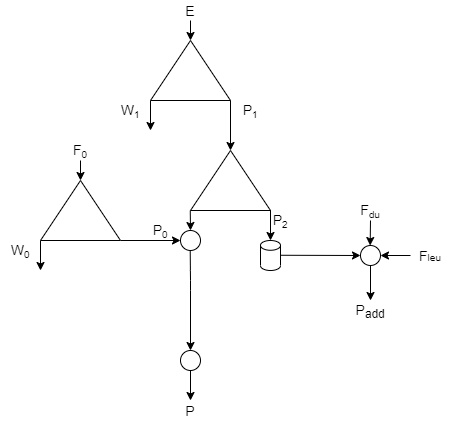
\includegraphics[scale=0.7]{cascades/P2utilization}}
  \caption{Схема независимого вовлечения загрязненногой изотопом $^{232}$U фракции с разбавлением обедненным и природным ураном}\label{P2utilization}
\end{figure}

Расчет целевых показателей схемы -- доли дополнительного НОУ-продукта, полученного из $P_2$, от новой ТВС (469 кг), а также экономии природного урана, производился на основе данных составов второго и пятого рециклов (см.постановку задачи), а также предположения двукратного увеличения предела содержания $^{232}$U в продукте, дополнительно произведенном из $P_2$ ($1\cdot10^{-7}$\% вместо $5\cdot10^{-7}$\%). Результаты вычислений представлены в таблице \ref{independent}.


\begin{table}[h]
  \centering
  \normalsize\begin{tabulary}{1.0\textwidth}{CCCCC}
  ПДК $^{232}$U & Цикл № & $P_2$, кг & Дополнительный продукт из $P_2$, доля новой ТВС, \% & Экономия природного урана, \% \\
  1.e-6\% & 2 & 1.09 & 7.11 & 14.6 \\
   & 5 & 0.92 & 10.21 & 6.3 \\
  5.e-7\% & 2 & 1.33 & 14.22 & 7.3 \\
   & 5 & 0.92 & 20.42 & 3.1 \\
  \end{tabulary}
  \caption{Результаты вовлечения $P_2$ в производство дополнительного НОУ-продукта. Обозначения: ПДК $^{232}$U -- предельно допустимая концентрация $^{232}$U в дополнительно производимом на основе $P_2$ продукте. {\label{independent}}}
\end{table}

Проведем анализ численных результатов расчета. Значения в столбце <<Дополнительный продукт из $P_2$, доля новой ТВС \%>> соответствуют доле дополнительно произведенного НОУ из побочного $P_2$, образовавшегося в процессе обогащения топлива из регенерата для одной ТВС (469 кг), а экономия природного урана приведена относительно схемы ординарного каскада для обогащения природного урана.

Как можно заключить из результатов, представленных в таблице \ref{independent}, предлагаемый способ использования $P_2$ через модификацию схемы двойного каскада с НОУ-разбавителем позволяет экономить дополнительное количество природного урана относительно двойного модифицированного каскада, в котором не предполагается задействование потока легкой фракции второго каскада. А эффект более значителен для случаев, когда задействуется побочный продукт $P_2$ двойного каскада, образующийся на начальных стадиях рециклирования уранового топлива. В рассматриваемом случае -- это второй рецикл (табл. \ref{independent}). Схема рис. \ref{P2utilization} также показывает себя как более предпочтительная в экономии природного урана (вдвое выигрышнее, согласно табл. \ref{independent}), когда предельно допустимая концентрация $^{232}$U в получаемом из $P_2$ конечном продукте допускается на уровне в два раза выше ($1\cdot10^{-7}$\% вместо $5\cdot10^{-7}$\%).  Значение экономии природного урана соответствует доле $P_2$, смешанной с обедненным ураном $F_{du}$, до того, как он будет смешан с НОУ-разбавителем $F_{leu}$, полученным из природного урана. Важно заметить, что значение этой доли соответствует экономии работы разделения, которая, в случае отказа от использования $P_2$, была бы затрачена на прямое обогащение природного урана в ординарном каскада для производства аналогичного замещающего количества свежего НОУ-продукта.

Итак, накопленный в ходе производства одной ТВС из регенерата побочный продукт $P_2$ можно использовать для производства дополнительных $\approx$7\% свежего НОУ-продукта от дополнительной топливной сборки. Это соответствует возможности произвести дополнительную 15-ю тепловыделяющую сборку из накопленного $P_2$, образовавшегося при производстве предыдущих четырнадцати ТВС. Таким образом, для современного легководного реактора, такого как, например, российский ВВЭР-1200 или европейский PWR, где активная зона состоит из более чем 150 тепловыделяющих сборок, взяв за основу предложенную схему, можно изготовить дополнительно более 10 ТВС. 



В качестве выводов, относящихся ко всем рассмотренным схемам, приведем следующие:
\begin{enumerate}
    \item схемы на основе двойного каскада, использующие НОУ-разбавитель, принципиально пригодны для решения задачи обогащения регенерированного урана в рамках многократного рецикла урановой составляющей топлива легководных реакторов. При этом каждая из схем имеет собственные достоинства и недостатки;
    \item характерным недостатком схемы, не предполагающей утилизацию нештатного отхода, образующегося в потоке $P_2$, является проблема с обращением с этим материалом, с высоким содержанием как четных изотопов (на 1-2 порядка выше, чем пределы для товарного НОУ) и $^{235}$U (до 20\% или, в некоторых случаях, до 90\%, в зависимости от выбранного режима работы каскадной схемы). Одним из вариантом обращения с ним, помимо схемы независимой утилизации побочного продукта легкой фракции второго каскада схемы двойного каскада с НОУ-разбавителем (рис. \ref{P2utilization}), может стать его перемешивание с отвалом первого каскада при обогащении регенерата. Оценки показали, что в этом случае возможно получить обедненный уран с приемлемым содержанием $^{232}$U (не выше $5\cdot10^{-7}$\%);
    \item характерными недостатком схемы двойного каскада с НОУ-разбавителем с возвратом потока $P_2$ в цикл (рис. \ref{P2utilizationRing}) является возврат значительной части четных изотопов на вход каскадной схемы;
    \item характерным недостатком схемы тройного каскада (рис. \ref{p2_withDepU}) являются дополнительные затраты работы разделения по отношению к схемам двойного каскада с НОУ-разбавителем, возникающие при обогащении разбавленного обедненным ураном отхода второго каскада схемы, загрязненного четными изотопами.
  \end{enumerate}

Анализ эффективности предложенных каскадных схем с точки зрения потерь $^{235}$U показал, что перспективными вариантами для дальнейшей технико-экономической проработки являются каскадные схемы двойного каскада с НОУ-разбавителем (рис. \ref{p2left}) и тройного каскада (рис. \ref{p2_withDepU}). Cхема двойного каскада с НОУ-разбавителем на каждом из рассмотренных рециклах позволяет извлечь более 80\% от массы $^{235}$U из исходного регенерированного урана, поступившего на обогащение.

Для каждой из предложенных схем разработаны оригинальные методики расчета и оптимизации ее переменных по критерию минимума расхода работы разделения каскадной схемы, основанная на использовании современных методов условной оптимизации функций многих переменных. С использованием разработанных методик расчета и оптимизации предложенных каскадных схем продемонстрирована возможность их использования для обогащения регенерированного урана в условиях многократного рецикла на примере взятого из литературы изотопного состава регенерата урана с повышенным содержанием четных изотопов и отвечающего пятому рециклу в топливе ВВЭР.

Для выбора конкретного варианта каскадной схемы для организации производственного процесса, необходим детальный технико-экономический анализ каждой из схем на основе их интегральных показателей, таких как расход сырьевых материалов и работы разделения, в контексте всей цепочки ядерного топливного цикла, а также с учетом возникающих в этой цепочке изменений при использовании регенерата урана по отношению к открытому топливному циклу. Помимо этого, необходима проработка технологических проблем каждой из схем, в частности, с точки зрения возможности эксплуатации и обслуживания оборудования в условиях работы с материалами, имеющими более высокую, чем природный уран удельную активность. Например, подобные условия возникают в каскадах, концентрирующие в легкой фракции $\alpha$-активные изотопы $^{232,234}$U.

\clearpage

